\documentclass[lang = cn, scheme = chinese, thmcnt = section, usesamecnt]{elegantbook}
% elegantbook      设置elegantbook文档类
% lang = cn        设置中文环境
% scheme = chinese 设置标题为中文
% thmcnt = section 设置计数器


%% 1.封面设置

\title{基础拓扑学讲义 - 尤承业 - 笔记}                % 文档标题

\author{若水}                        % 作者

\myemail{ethanmxzhou@163.com}       % 邮箱

\homepage{helloethanzhou.github.io} % 主页

\date{\today}                       % 日期

\logo{PiCreatures_happy.pdf}        % 设置Logo

\cover{阿基米德螺旋曲线.pdf}          % 设置封面图片

% 修改标题页的色带
\definecolor{customcolor}{RGB}{135, 206, 250} 
% 定义一个名为customcolor的颜色,RGB颜色值为(135, 206, 250)

\colorlet{coverlinecolor}{customcolor}     % 将coverlinecolor颜色设置为customcolor颜色

%% 2.目录设置
\setcounter{tocdepth}{3}  % 目录深度为3

%% 3.引入宏包
\usepackage[all]{xy}
\usepackage{bbm, svg, graphicx, float, extpfeil, amsmath, amssymb, mathrsfs, mathalpha, hyperref, centernot}


%% 4.定义命令
\newcommand{\N}{\mathbb{N}}            % 自然数集合
\newcommand{\R}{\mathbb{R}}            % 实数集合
\newcommand{\C}{\mathbb{C}}  		   % 复数集合
\newcommand{\Q}{\mathbb{Q}}            % 有理数集合
\newcommand{\Z}{\mathbb{Z}}            % 整数集合
\newcommand{\sub}{\subset}             % 包含
\newcommand{\im}{\text{im }}           % 像
\newcommand{\lang}{\langle}            % 左尖括号
\newcommand{\rang}{\rangle}            % 右尖括号
\newcommand{\bs}{\boldsymbol}          % 向量加黑
\newcommand{\pll}{\kern 0.56em/\kern -0.8em /\kern 0.56em} % 平行
% \newcommand{\dd}{\mathrm{d}}           % 微分d
\newcommand{\dis}{\displaystyle}
\newcommand{\function}[5]{
	\begin{align*}
		#1:\begin{aligned}[t]
			#2 &\longrightarrow #3\\
			#4 &\longmapsto #5
		\end{aligned}
	\end{align*}
}                                     % 函数

\newcommand{\lhdneq}{%
	\mathrel{\ooalign{$\lneq$\cr\raise.22ex\hbox{$\lhd$}\cr}}} % 真正规子群

\newcommand{\rhdneq}{%
	\mathrel{\ooalign{$\gneq$\cr\raise.22ex\hbox{$\rhd$}\cr}}} % 真正规子群

\begin{document}

\maketitle       % 创建标题页

\frontmatter     % 开始前言部分

\chapter*{致谢}

\markboth{致谢}{致谢}

\vspace*{\fill}
	\begin{center}
		
		\large{感谢 \textbf{ 勇敢的 } 自己}
		
	\end{center}
\vspace*{\fill}

\tableofcontents % 创建目录

\mainmatter      % 开始正文部分

\chapter{拓扑空间}

\section{拓扑空间}

\subsection{拓扑定义}

\begin{definition}{拓扑}
	对于集合$X$,称子集族$\tau\sub\mathscr{P}(X)$为$X$的拓扑,如果成立如下命题。
	\begin{enumerate}
		\item $\varnothing,X\in \tau$
		\item 若$A,B\in \tau$,则$A\cap B\in\tau$。
		\item 若$\{ A_\lambda \}_{\lambda\in\Lambda}\sub \tau$,则$\dis\bigcup_{\lambda\in\Lambda}A_\lambda\in\tau$。
	\end{enumerate}
\end{definition}

\begin{example}
	\begin{enumerate}
		\item 平凡拓扑:$\{\varnothing,X\}$
		\item 离散拓扑:$2^X=\mathscr{P}(X)$
		\item 余有限拓扑:对于无穷集合$X$,则称$X$上的余有限拓扑为
		$$
		\tau_f=\{A:A^c\sub X\text{为有限子集}\}\cup\{\varnothing\}
		$$
		\item 余可数拓扑:对于不可数无穷集合$X$,则称$X$上的余可数拓扑为
		$$
		\tau_c=\{A:A^c\sub X\text{为可数子集}\}\cup\{\varnothing\}
		$$
		\item 欧式拓扑:称$\R^n$上的欧式拓扑为
		$$
		E^n=\{U\sub\R^n:U\text{为开方体的并}\}
		$$
		\item 度量拓扑:对于度量空间$(X,d)$,则称$X$上由$d$诱导的拓扑为
		$$
		\tau_d=\{ U:U\text{为若干开球的并} \}
		$$
	\end{enumerate}
\end{example}

\begin{definition}{开集}
	称拓扑空间的元素为开集。
\end{definition}

\begin{proposition}{开集的性质}
	\begin{enumerate}
		\item $\varnothing,X$为开集。
		\item 任意开集的并为开集。
		\item 有限开集的交为开集。
	\end{enumerate}
\end{proposition}

\begin{definition}{闭集}
	称开集的补集为闭集。
\end{definition}

\begin{proposition}{闭集的性质}
	\begin{enumerate}
		\item $\varnothing,X$为闭集。
		\item 任意闭集的交为闭集。
		\item 有限闭集的并为闭集。
		\item {\bf 分离定理}:在度量空间$(X,d)$中,如果闭集$E\cap F=\varnothing$,那么$d(E,F)>0$。
	\end{enumerate}
\end{proposition}

\subsection{拓扑结构}

\begin{definition}{开集}
	称集合$X$的子集族$\mathscr{G}\sub\mathscr{P}(X)$中的元素为开集,如果成立如下开集公理。
	\begin{enumerate}
		\item $\varnothing,X\in\mathscr{G}$
		\item 有限交封闭:如果$G_1,G_2\in\mathscr{G}$,那么$G_1\cap G_2\in\mathscr{G}$。
		\item 任意并封闭:如果$\{ G_\lambda \}\sub\mathscr{G}$,那么$\bigcup G_\lambda\in\mathscr{G}$。
	\end{enumerate}
\end{definition}

\begin{definition}{闭集}
	称集合$X$的子集族$\mathscr{F}\sub\mathscr{P}(X)$中的元素为闭集,如果成立如下闭集公理。
	\begin{enumerate}
		\item $\varnothing,X\in\mathscr{F}$
		\item 有限交封闭:如果$F_1,F_2\in\mathscr{F}$,那么$F_1\cap F_2\in\mathscr{F}$。
		\item 任意并封闭:如果$\{ F_\lambda \}\sub\mathscr{F}$,那么$\bigcup F_\lambda\in\mathscr{F}$。
	\end{enumerate}
\end{definition}

\begin{definition}{开核}
	对于集合$X$,称算子$\mathcal{O}:\mathscr{P}(X)\to\mathscr{P}(X)$为开核算子,$\mathcal{O}(E)$称为$E$的开核,如果成立如下开核公理。
	\begin{enumerate}
		\item 幂等性:$\mathcal{O}^2=\mathcal{O}$
		\item 包含的单调性:如果$E\sub F$,那么$\mathcal{O}(E)\sub \mathcal{O}(F)$。
		\item 交的分配律:如果$E\sub F$,那么$\mathcal{O}(E\cap F)=\mathcal{O}(E)\cap \mathcal{O}(F)$。
	\end{enumerate}
\end{definition}

\begin{definition}{闭包}
	对于集合$X$,称算子$\mathcal{C}:\mathscr{P}(X)\to\mathscr{P}(X)$为闭包算子,$\mathcal{C}(E)$称为$E$的闭包,如果成立如下闭包公理。
	\begin{enumerate}
		\item 幂等性:$\mathcal{C}^2=\mathcal{C}$
		\item 包含的单调性:如果$E\sub F$,那么$\mathcal{C}(E)\sub \mathcal{C}(F)$。
		\item 并的分配律:如果$E\sub F$,那么$\mathcal{C}(E\cup F)=\mathcal{C}(E)\cup \mathcal{C}(F)$。
	\end{enumerate}
\end{definition}

\begin{definition}{邻域}
	对于集合$X$,称算子$\mathcal{U}:X\to\mathscr{P}(\mathscr{P}(X))$为邻域算子,$\mathcal{U}(x)$称为$x$的邻域系,$\mathcal{U}(x)$中的元素称为$x$的邻域,如果成立如下邻域公理。
	\begin{enumerate}
		\item 如果$U\in \mathcal{U}(x)$,那么$x\in U$。
		\item 如果$U,V\in\mathcal{U}(x)$,那么$U\cap V\in\mathcal{U}(x)$。
		\item 如果$U\in \mathcal{U}(x)$且$U\sub V$,那么$V\in\mathcal{U}(x)$。
		\item 对于任意$U\in\mathcal{U}(x)$,存在$V\in\mathcal{U}(x)$,使得对于任意$v\in V$,成立$U\in\mathcal{U}(v)$。
	\end{enumerate}
\end{definition}

\subsection{拓扑中点的结构}

\begin{definition}{内点}
	对于拓扑空间$X$,称点$x$为子集$A$的内点,如果成立如下命题之一。
	\begin{enumerate}
		\item 存在开集$U$,使得成立$x\in U\sub A$。
		\item $x\in A^\circ$
	\end{enumerate}
\end{definition}

\begin{definition}{接触点}
	对于拓扑空间$X$,称点$x$为子集$A$的接触点,如果成立如下命题之一。
	\begin{enumerate}
		\item 对于任意$x$的邻域$U$,成立$U\cap A\ne\varnothing$。
		\item $x\in \overline{A}$
	\end{enumerate}
\end{definition}

\begin{definition}{边界点}
	对于拓扑空间$X$,称点$x$为子集$A$的边界点,如果对于任意$x$的邻域$U$,成立%
	$$
	A\cap U\ne\varnothing,\qquad
	U\setminus A\ne\varnothing
	$$
\end{definition}

\begin{definition}{聚点}
	对于拓扑空间$X$,称点$x$为子集$A$的聚点,如果成立如下命题之一。
	\begin{enumerate}
		\item 对于任意$x$的邻域$U$,成立$U\cap A\setminus\{x\}\ne\varnothing$。
		\item $x\in A'$
	\end{enumerate}
\end{definition}

\begin{definition}{孤立点}
	对于拓扑空间$X$,称点$x$为子集$A$的孤立点,如果存在$x$的邻域$U$,使得成立%
	$$
	A\cap U=\{ x \}
	$$
\end{definition}

\subsection{拓扑中集合的结构}

\begin{definition}{邻域}
	\begin{enumerate}
		\item 对于拓扑空间$X$,称子集$U$为点$x$的邻域,如果成立如下命题之一。
		\begin{enumerate}
			\item 存在开集$G$,使得成立$x\in G\sub U$。
			\item $x\in U^\circ$
		\end{enumerate}
		\item 对于拓扑空间$X$,称子集$U$为子集$A$的邻域,如果成立如下命题之一。
		\begin{enumerate}
			\item 存在开集$G$,使得成立$A\sub G\sub U$。
			\item $A\sub U^\circ$
		\end{enumerate}
	\end{enumerate}
\end{definition}

\begin{definition}{内部}
	\begin{enumerate}
		\item 对于拓扑空间$X$,称子集$A$的内点全体为$A$的内部,记作$A^\circ$。
		\item 对于拓扑空间$X$,定义子集$A$的内部为包含于$A$的极大开集,换言之%
		$$
		A^\circ=\bigcup_{G\sub A\text{为开集}}G
		$$
	\end{enumerate}
\end{definition}

\begin{proposition}{内部的性质}
	\begin{enumerate}
		\item 如果$A\sub B$,那么$A^\circ\sub B^\circ$。
		\item $A^\circ=A\iff A$为开集。
		\item $(A\cap B)^\circ=A^\circ\cap B^\circ$
		\item $(A\cup B)^\circ \supset A^\circ\cup B^\circ$
		\item 反例:$((-1,0]\cup[0,1))^\circ\supsetneq (-1,0]^\circ\cup[0,1)^\circ$
	\end{enumerate}
\end{proposition}

\begin{definition}{闭包}
	\begin{enumerate}
		\item 对于拓扑空间$X$,称子集$A$的接触点全体为$A$的闭包,记作$\overline{A}$。
		\item 对于拓扑空间$X$,定义子集$A$的闭包为包含$A$的极小闭集,换言之%
		$$
		\overline{A}=\bigcap_{F\supset A\text{为闭集}}F
		$$
	\end{enumerate}
\end{definition}

\begin{proposition}{闭包的性质}
	\begin{enumerate}
		\item 如果$A\sub B$,那么$\overline{A}\sub \overline{B}$。
		\item $\overline{A}=A\iff A$为闭集。
		\item $\overline{A\cup B}=\overline{A}\cup \overline{B}$
		\item $\overline{A\cap B}\sub\overline{A}\cap \overline{B}$
		\item 反例:$\overline{(-1,0)\cap (0,1)}\subsetneq\overline{(-1,0)}\cap \overline{(0,1)}$
	\end{enumerate}
\end{proposition}

\begin{definition}{边界}
	对于拓扑空间$X$,称子集$A$的边界点全体为$A$的边界,记作$\partial A$。
\end{definition}

\begin{definition}{导集}
	对于拓扑空间$X$,称子集$A$的聚点全体为$A$的导集,记作$A'$。
\end{definition}

\begin{proposition}{导集的性质}
	\begin{enumerate}
		\item 如果$A\sub B$,那么$A'\sub B'$。
		\item $(A\cup B)'=A'\cup B'$
	\end{enumerate}
\end{proposition}

\begin{definition}{孤立点集}
	对于拓扑空间$X$,称子集$A$的孤立点全体为$A$的孤立点集,记作$A^i$。
\end{definition}

\begin{theorem}
	\begin{enumerate}
		\item 内部与闭包的关系:%
		$$
		(A^c)^\circ=(\overline{A})^c
		$$
		\item 闭包的分割:%
		$$
		\overline{A}
		=A^\circ\sqcup \partial A
		=A^i\sqcup A'
		$$
		\item 全空间的分割:%
		$$
		X
		=A^\circ\sqcup\partial A\sqcup(A^c)^\circ
		=A^\circ\sqcup\partial\sqcup(\overline{A})^c
		$$
	\end{enumerate}
\end{theorem}

\subsection{拓扑结构}

\begin{definition}{稠密集}
	对于拓扑空间$X$,称子集$A$为稠密集,如果$\overline{A}=X$。
\end{definition}

\begin{example}
	\begin{enumerate}
		\item $(\R,\tau_f)$的任意无穷子集是稠密的。
		\item $(\R,\tau_c)$的任意可数子集不是稠密的。
	\end{enumerate}
\end{example}

\begin{definition}{无处稠密集}
	对于拓扑空间$X$,称子集$A$为无处稠密集,如果$(\overline{A})^\circ=\varnothing$。
\end{definition}

\begin{definition}{可分空间}
	称拓扑空间$X$为可分空间,如果$X$存在可数稠密子集。
\end{definition}

\begin{example}
	\begin{enumerate}
		\item $(\R,\tau_f)$是可分的。
		\item $(\R,\tau_c)$不是可分的。
	\end{enumerate}
\end{example}

\begin{definition}{收敛}
	对于拓扑空间$X$,称序列$\{x_n\}_{n=1}^{\infty}$收敛于点$x$,并记作$x_n\to x$。,如果对于$x$的任意邻域$U$,存在$N\in\N^*$,使得对于任意$n>N$,成立$x_n\in U$。
\end{definition}

\begin{remark}
	极限不唯一:在$(\R,\tau_f)$中,对于两两互异序列$\{x_n\}$,以及任意$x\in\R$,由于$x$的任意邻域(有限集的补集)包含$\{x_n\}$的几乎所有项,于是$x_n\to x$。
\end{remark}

\begin{remark}
	聚点存在定理(聚点则存在收敛于其的序列)不成立:在$(\R,\tau_c)$中,由于$x_n\to x\implies$对于几乎所有$x_n$成立$x_n=x$,那么令$A$不可数,于是$\overline{A}=\R$(包含$A$的闭集且不可数的只有$\R$),取$x\notin A$,那么$x$为$A$的聚点,但是$A$中任意序列不可能收敛于$x$
\end{remark}

\subsection{拓扑子空间}

\begin{definition}{子空间}
	对于拓扑空间$(X,\tau)$,拓扑$\tau_A=\{ U\cap A:U\in\tau \}$为由$\tau$诱导的子集$A$上的子空间拓扑,称$(A,\tau_A)$为$(X,\tau)$的子空间。
\end{definition}

\begin{proposition}{子空间的性质}
	\begin{enumerate}
		\item 对于拓扑空间以及$B\sub A \sub X$,成立$(\tau_A)_B=\tau_B$
		\item 对于度量拓扑空间$(X,\tau_d)$以及$A\sub X$,成立$\tau_{d_A}=\tau_{d|_A}$。
	\end{enumerate}
\end{proposition}

\begin{remark}
	开集具有相对性,例如$(0,1)$是$E^1$上的开集,但不是$E^2$上的开集。
\end{remark}

\begin{theorem}{开闭集的相对性}
	对于拓扑空间$X$,以及子集$B\sub A$,成立如下命题。
	\begin{enumerate}
		\item $B$为$A$的开/闭集$\iff$存在$X$的开/闭集$C\sub X$,使得成立$B=A\cap C$。
		\item 如果$B$为$X$的开/闭集,那么$B$亦为$A$的开/闭集。
		\item 如果$B$为$A$的开/闭集,且$A$为$X$的开/闭集,那么$B$亦为$X$的开/闭集。
	\end{enumerate}
\end{theorem}

\section{连续映射与同胚映射}

\subsection{连续映射}

\begin{definition}{连续}
	对于拓扑空间$X$与$Y$,称映射$f:X\to Y$在点$x$处连续,如果对于$f(x)$中的任意邻域$V$,$f^{-1}(V)$为$x$的邻域。
\end{definition}

\begin{definition}{序列连续}
	对于拓扑空间$X$与$Y$,称映射$f:X\to Y$在点$x$处序列连续,如果对于任意序列$x_n\to x$,成立$f(x_n)\to f(x)$。
\end{definition}

\begin{definition}{连续映射}
	对于拓扑空间$X$与$Y$,称映射$f:X\to Y$为连续映射,如果成立如下命题之一。
	\begin{enumerate}
		\item 邻域的原像为邻域。
		\item 开集的原像为开集。
		\item 闭集的原像为闭集。
	\end{enumerate}
\end{definition}

\begin{proposition}{连续映射的封闭性}
	连续映射对于四则运算与复合运算封闭。
\end{proposition}

\begin{definition}{拓扑性在连续映射下的像}
	\begin{enumerate}
		\item 紧致空间在连续映射下的像为紧致空间。
		\item 连通空间在连续映射下的像为连通空间。
		\item 道路连通空间在连续映射下的像为道路连通空间。
	\end{enumerate}
\end{definition}

\begin{theorem}{局部连续与全局连续}
	对于拓扑空间$X$与$Y$,以及映射$f:X\to Y$,定义$f$在子集$A$上的限制为$f|_A:A\to Y$,那么成立如下命题。
	\begin{enumerate}
		\item 若$f$在点$x$处连续,则$f_A$在点$x$处连续。
		\item 若$A$为点$x$的邻域,且$f|_A$在点$x$处连续,则$f$在$x$处连续。
	\end{enumerate}
\end{theorem}

\begin{definition}{覆盖}
	\begin{enumerate}
		\item 对于拓扑空间$X$,称$\mathscr{C}\sub \mathscr{P}(X)$为$X$的覆盖,如果$\displaystyle X=\bigcup_{C\in\mathscr{C}}C$。
		\item 对于拓扑空间$X$,称$\mathscr{C}\sub \mathscr{P}(X)$为子集$A$的覆盖,如果$\displaystyle A\sub \bigcup_{C\in\mathscr{C}}C$。
	\end{enumerate}
\end{definition}

\begin{theorem}{粘接引理}{粘接引理}
	对于拓扑空间$X$的有限闭覆盖$\{A_k\}_{k=1}^{n}$,如果诸映射$f|_{A_k}:A_k\to Y$均为连续映射,那么$f:X\to Y$为连续映射。
\end{theorem}

\subsection{同胚映射}

\begin{definition}{同胚映射}
	对于拓扑空间$X$与$Y$,称双射$f:X\to Y$为同胚映射,如果$f$与$f^{-1}$均为连续映射。
\end{definition}

\begin{definition}{嵌入映射}
	对于拓扑空间$X$与$Y$,称连续映射$f:X\to Y$为嵌入映射,如果映射$f:X\to f(X)$为同胚映射。
\end{definition}

\begin{definition}{同胚}
	称拓扑空间$X$与$Y$同胚,并记作$X\cong Y$,如果存在同胚映射$f:X\to Y$。
\end{definition}

引入记号:%
$$
D^n=\{ x\in E^n:\Vert x \Vert\le 1 \},\qquad 
S^{n}=\{ x\in E^{n+1}:\Vert x \Vert= 1 \}
$$

\begin{example}
	$(-1,1)\cong (-1,1)$:
	\begin{align*}
		(-1,1) &\longrightarrow (-1,1)\\
		x &\longmapsto \tan\frac{\pi}{2}x
	\end{align*}
\end{example}

\begin{example}
	$E^n\cong D^n\setminus S^{n-1}$:%
	\begin{align*}
		E^n &\longrightarrow D^n\setminus S^{n-1}\\
		x &\longmapsto \frac{x}{1+\|x\|}
	\end{align*}
\end{example}

\begin{example}
	$E^n\setminus\{O\}\cong E^n\setminus D^n$:%
	\begin{align*}
		E^n &\longrightarrow D^n\setminus S^{n-1}\\
		x &\longmapsto x+\frac{x}{\|x\|}
	\end{align*}
\end{example}

\begin{example}
	$S^2\setminus \{ \mathcal{N} \} \cong E^2$:定义Riemann球面
	$$
	\mathbb{S}=\left\{ (X,Y,Z):X^2+Y^2+\left(Z-\frac{1}{2}\right)^2=\frac{1}{4} \right\}
	$$
	Riemann球面的北极记作$\mathcal{N}=(0,0,1)$,那么存在同胚映射
	\begin{align*}
		\mathcal{R}:\begin{aligned}[t]
			\mathbb{S}\setminus \{ \mathcal{N} \} &\longrightarrow \C\\
			(x,y,z) &\longmapsto \left(\frac{x}{1-z},\frac{y}{1-z}\right)
		\end{aligned}
	\end{align*}
	与
	\begin{align*}
		\mathcal{R}^{-1}:\begin{aligned}[t]
			\C &\longrightarrow \mathbb{S}\setminus \{ \mathcal{N} \}\\
			(x,y) &\longmapsto \left( \frac{2x}{1+x^2+y^2},\frac{2y}{1+x^2+y^2},1-\frac{2}{1+x^2+y^2} \right)
		\end{aligned}
	\end{align*}
	从而$\mathbb{S}\setminus \{ \mathcal{N} \} \cong \C$;换言之,$S^2\setminus \{ \mathcal{N} \} \cong E^2$。
\end{example}

\section{乘积空间与拓扑基}

\begin{definition}{生成子集族}
	对于集合$X$的子集族$\mathscr{B}\sub\mathscr{P}(X)$,定义由$\mathscr{B}$生成的子集族为
	\begin{align*}
		\overline{\mathscr{B}}&=\{ U\sub X:U\text{为}\mathscr{B}\text{中集合的并} \}\\
		&=\{ U\sub X:\forall x\in U,\exists B\in\mathscr{B},x\in B\sub U \}
	\end{align*}
\end{definition}

\begin{definition}{投影}
	对于集合$X$与$Y$,定义其投影为
	\begin{align*}
		j_x: & X\times Y\to X\\
		& (x,y)\to x
	\end{align*}
	\begin{align*}
		j_y: & X\times Y\to Y\\
		& (x,y)\to y
	\end{align*}
\end{definition}

\subsection{乘积空间}

\begin{definition}{乘积拓扑}
	对于拓扑空间$(X,\tau)$与$(Y,\upsilon)$,令$\mathscr{B}=\{ U\times V :U\in\tau,V\in\upsilon \}$,称$\overline{\mathscr{B}}$为$X\times Y$上的乘积拓扑,$(X\times Y,\overline{\mathscr{B}})$为$(X,\tau)$与$(Y,\upsilon)$的乘积空间。
\end{definition}

\begin{proposition}
	\begin{enumerate}
		\item $\overline{\mathscr{B}}$为$X\times Y$上的一个拓扑。
		\item 映射$f:X\to Y\times Z$连续$\iff$映射$j_y\circ f$与$j_z\circ f$连续。
	\end{enumerate}
\end{proposition}

\subsection{拓扑基}

\begin{definition}{拓扑基}
	称集合$X$的子集族$\mathscr{B}\sub\mathscr{P}(X)$为集合$X$的拓扑基,如果成立如下命题之一。
	\begin{enumerate}
		\item $\overline{\mathscr{B}}$为$X$的一个拓扑。
		\item $\displaystyle\bigcup_{B\in\mathscr{B}}B=X$,且对于任意$B_1,B_2\in\mathscr{B}$,成立$B_1\cap B_2\in\overline{\mathscr{B}}$。
		\item $\displaystyle\bigcup_{B\in\mathscr{B}}B=X$,且对于任意$B_1,B_2\in\mathscr{B}$,以及任意$x\in B_1\cap B_2$,存在$B\in\mathscr{B}$,使得成立$x\in B\sub B_1\cap B_2$。
	\end{enumerate}
\end{definition}

\begin{definition}{拓扑空间的拓扑基}
	称集合$X$的子集族$\mathscr{B}\sub\mathscr{P}(X)$为拓扑空间$(X,\tau)$的拓扑基,如果成立如下命题之一。
	\begin{enumerate}
		\item $\overline{\mathscr{B}}=\tau$
		\item $\mathscr{B}\sub \tau \sub \overline{\mathscr{B}}$
	\end{enumerate}
\end{definition}

\begin{theorem}
	如果$\mathscr{B}$为拓扑空间$(X,\tau)$的拓扑基,那么成立如下命题。
	\begin{enumerate}
		\item $x\in A^\circ\iff$存在$B\in\mathscr{B}$,使得成立$x\in B\sub A$。
		\item $x\in A'\iff$对于任意$B\in\mathscr{B}$,若$x\in B$,则$A\cap B\setminus\{x\}\ne\varnothing$。
		\item $x\in \overline{A}\iff$对于任意$B\in\mathscr{B}$,若$x\in B$,则$A\cap B\ne\varnothing$。
		\item 映射$f:Y\to X$连续$\iff$对于任意$B\in\mathscr{B}$,$f^{-1}(B)$为$Y$的开集。
	\end{enumerate}
\end{theorem}

\section{同胚不变性,遗传性与可乘性}

\begin{definition}{拓扑概念与拓扑性质}
	\begin{enumerate}
		\item 称拓扑空间在同胚映射下保持不变的概念为拓扑概念。
		\item 称拓扑空间在同胚映射下保持不变的性质为拓扑性质。
	\end{enumerate}
\end{definition}

\begin{definition}{遗传性}
	称拓扑性质$P$具有遗传性,如果若拓扑空间$X$成立$P$,则其任意子空间$A$亦成立$P$。
\end{definition}

\begin{definition}{可乘性}
	称拓扑性质$P$具有可乘性,如果若拓扑空间$X$与$Y$成立$P$,则其乘积空间$X\times Y$也成立$P$。
\end{definition}

\begin{table}[H]
	\centering
	\caption{拓扑性质的遗传性与可乘性}
	\renewcommand{\arraystretch}{1.25}
	\begin{tabular}{>{\centering\arraybackslash}m{2cm}>{\centering\arraybackslash}m{2cm}>{\centering\arraybackslash}m{2cm}}
		\toprule
		\textbf{拓扑性质} & \textbf{遗传性} & \textbf{可乘性} \\
		\midrule
		$T_1$公理 & $\checkmark$ & $\checkmark$ \\
		$T_2$公理 & $\checkmark$ & $\checkmark$ \\
		$T_3$公理 & $\checkmark$ & $\checkmark$ \\
		$T_4$公理 & $\times$     & $\times$     \\
		$C_1$公理 & $\checkmark$ & $\checkmark$ \\
		$C_2$公理 & $\checkmark$ & $\checkmark$ \\
		可分性    & $\checkmark$ & $\times$   \\
		紧致性    & $\times$     & $\checkmark$ \\
		列紧性    &              &              \\
		连通性    & $\times$     & $\checkmark$ \\
		道路连通性    & $\times$     & $\checkmark$ \\
		\bottomrule
	\end{tabular}
\end{table}

\chapter{拓扑性质}

\section{分离公理与可数公理}

\subsection{分离公理}

\begin{definition}{$T_0$公理}
	称拓扑空间$X$成立$T_0$公理,如果对于任意点$x\ne y$,存在开集$U$,使得成立或$x\in U$且$y\notin U$,或$y\in U$且$x\notin U$。
\end{definition}

\begin{definition}{$T_1$公理}
	称拓扑空间$X$成立$T_1$公理,如果成立如下命题之一。
	\begin{enumerate}
		\item 对于任意点$x\ne y$,存在$x$的邻域$U$与$y$的邻域$V$,使得成立$x\notin V$且$y\notin U$。
		\item 对于任意点$x$,子集$\{x\}$为闭集。
	\end{enumerate}
\end{definition}

\begin{definition}{$T_2$公理}
	称拓扑空间$X$成立$T_2$公理,如果成立如下命题之一。
	\begin{enumerate}
		\item 对于任意点$x\ne y$,存在$x$的邻域$U$与$y$的邻域$V$,使得成立$U\cap V=\varnothing$。
		\item $\Delta=\{ (x,x):x\in X \}$为$X\times X$的闭集。
	\end{enumerate}
\end{definition}

\begin{definition}{$T_3$公理}
	称拓扑空间$X$成立$T_3$公理,如果成立如下命题之一。
	\begin{enumerate}
		\item 对于任意点$x$与闭集$F$,若$x\notin F$,则存在$x$的邻域$U$与$F$的邻域$V$,使得成立$U\cap V=\varnothing$。
		\item 对于任意点$x$与$x$的开邻域$U$,存在$x$的开邻域$V$,使得成立$\overline{V}\sub U$。
	\end{enumerate}
\end{definition}

\begin{definition}{$T_4$公理}
	称拓扑空间$X$成立$T_4$公理,如果成立如下命题之一。
	\begin{enumerate}
		\item 对于任意不交闭集$E,F$,存在$E$的邻域$U$与$F$的邻域$V$,使得成立$U\cap V=\varnothing$。
		\item 对于任意闭集$F$与$F$的开邻域$U$,存在$F$的开邻域$V$,使得成立$\overline{V}\sub U$。
	\end{enumerate}
\end{definition}

\begin{definition}{Hausdorff空间}
	称成立$T_2$公理的拓扑空间为Hausdorff空间。
\end{definition}

\begin{theorem}{分离公理间的关系}
	$$
	T_2\implies T_1,\qquad
	T_0+T_3\implies T_2,\qquad
	T_1+T_3\implies T_2,\qquad
	T_1+T_4\implies T_3
	$$
\end{theorem}

\begin{proposition}
	如果拓扑空间$X$成立$T_1$公理,且点$x$为子集$A$的聚点,那么对于$x$的任意邻域$U$,$A\cap U$为无穷集。
\end{proposition}

\begin{theorem}{Hausdorff空间中的唯一收敛性}
	在Hausdorff空间中,收敛点列存在且存在唯一极限。
\end{theorem}

\begin{theorem}{度量空间}
	度量空间$(X,d)$成立$T_1,T_2,T_3,T_4,C_1$公理。
\end{theorem}

\subsection{可数公理}

\begin{definition}{邻域系}
	对于拓扑空间$X$,称点$x$的邻域全体为$x$的邻域系,记作$\mathscr{N}(x)$。
\end{definition}

\begin{definition}{邻域基}
	对于拓扑空间$X$,称$\mathscr{U}\sub\mathscr{N}(x)$为点$x$的邻域基,如果对于任意$N\in\mathscr{N}(x)$,存在$U\in\mathscr{U}$,使得成立$U\sub N$。
\end{definition}

\begin{example}
	\begin{enumerate}
		\item 邻域系为邻域基。
		\item 开邻域系为邻域基。
		\item 如果$\mathscr{B}$为拓扑基,那么$\mathscr{U}=\{ B\in\mathscr{B}:x\in B \}$为$x$的邻域基。
	\end{enumerate}
\end{example}

\begin{definition}{$C_1$公理}
	称拓扑空间成立$C_1$公理,如果其中任意一点处存在可数邻域基。
\end{definition}

\begin{theorem}{嵌套定理}
	对于拓扑空间,如果某点处存在可数邻域基,那么该点处存在单调递减的可数邻域基。
\end{theorem}

\begin{theorem}{聚点定理}
	如果拓扑空间$X$为$C_1$空间,且$x\in \overline{A}$,那么存在序列$\{ x_n \}_{n=1}^{\infty}\sub A$,使得成立$x_n\to x$。
\end{theorem}

\begin{theorem}{Heine定理/归结原理}
	$C_1$空间中序列连续与连续等价;换言之,对于$C_1$空间$X$以及映射$f:X\to Y$,$f$在$x$处连续$\iff$对于任意序列$x_n\to x$,成立$f(x_n)\to f(x)$。
\end{theorem}

\begin{definition}{$C_2$公理}
	称拓扑空间成立$C_2$公理,如果其存在可数拓扑基。
\end{definition}

\begin{theorem}{$C_2\implies C_1$}
	如果拓扑空间$X$为$C_2$空间,那么其为$C_1$空间。
\end{theorem}

\begin{proof}
	由于$X$为$C_2$空间,那么$X$存在可数拓扑基$\{B_n\}_{n=1}^{\infty}$。任取点$x$,断言:$\mathscr{U}=\{ B_n:x\in B_n,n\in\N^* \}$为$X$的可数邻域基。因此$X$为$C_1$空间。
\end{proof}

\begin{theorem}{$C_2\implies$可分}
	如果拓扑空间$X$为$C_2$空间,那么其为可分空间。
\end{theorem}

\begin{proof}
	由于$X$为$C_2$空间,那么$X$存在可数拓扑基$\{B_n\}_{n=1}^{\infty}$。在诸$B_n$中任取点$x_n$,断言:$\{x_n\}_{n=1}^{\infty}$为$X$的可数稠密子集。因此$X$为$C_1$空间。
\end{proof}

\begin{theorem}{可分度量空间$\implies C_2$}
	如果拓扑空间$X$为可分度量空间,那么其为$C_2$空间。
\end{theorem}

\begin{proof}
	由于$X$为可分空间,那么$X$存在可数稠密子集$\{x_n\}_{n=1}^{\infty}$。断言:$\dis \bigcup_{m,n=1}^{\infty}B_{1/m}(x_n)$为$X$的可数拓扑基。因此$X$为$C_2$空间。
\end{proof}

\section{Urysohn引理}

\begin{theorem}{Urysohn引理}
	如果拓扑空间$X$成立$T_4$公理,那么对于任意不交闭集$A,B$,存在连续映射$f:X\to E^1$,使得成立$f(A)=\{0\}$且$f(B)=\{1\}$。
\end{theorem}

\begin{theorem}{Tietze扩张定理}
	如果拓扑空间$X$成立$T_4$公理,那么对于任意闭集$F$与连续映射$f:F\to E^1$,存在连续映射$\tilde{f}:X\to E^1$,使得$\tilde{f}|_F=f$。
\end{theorem}

\begin{definition}{可度量化}
	称拓扑空间$(X,\tau)$可度量化,如果成立如下命题之一。
	\begin{enumerate}
		\item 存在度量$d:X\times X\to X$,使得成立$\tau_d=\tau$。
		\item 存在度量空间$(Y,d)$,以及嵌入映射$f:(X,\tau)\to(Y,d)$。
	\end{enumerate}
\end{definition}

\begin{theorem}{Urysohn度量化定理}
	如果拓扑空间成立$T_1,T_4$与$C_2$公理,那么其可嵌入Hilbert空间中。
\end{theorem}

\section{紧致性}

\subsection{完全有界性}

\begin{definition}{$\delta$-网}
	对于度量空间$(X,d)$,称子集$A$为$X$的$\delta$-网,如果$\displaystyle\bigcup_{a\in A}B_\delta(a)=X$。
\end{definition}

\begin{definition}{完全有界性}
	称度量空间为完全有界的,如果对于任意$\delta>0$,其存在有限$\delta$-网。
\end{definition}

\begin{definition}{Lebesgue数}
	对于列紧度量空间$(X,d)$,若$X$的开覆盖$\mathscr{U}$成立$X\notin \mathscr{U}$,则定义$\mathscr{U}$的Lebesgue数为%
	$$
	L_X(\mathscr{U})=\inf_{x\in X}\sup_{U\in\mathscr{U}}\inf_{u\in U^c}d(x,u)
	$$
\end{definition}

\begin{proposition}
	对于列紧度量空间$(X,d)$,如果$X$的开覆盖$\mathscr{U}$成立$X\notin \mathscr{U}$,且$L_X(\mathscr{U})>0$,同时对于任意$\delta\in(0,L_X(\mathscr{U}))$与$x\in X$,存在$U\in\mathscr{U}$,使得成立$B_\delta(x)\sub U$。
\end{proposition}

\subsection{列紧性与紧致性}

\begin{definition}{列紧性}
	称拓扑空间为列紧空间,如果其任意序列存在收敛子序列。
\end{definition}

\begin{definition}{紧致性}
	称拓扑空间为紧致空间,如果其任意开覆盖存在有限子覆盖。
\end{definition}

\begin{theorem}{完全有界性,列紧性与紧致性的关系}
	\begin{enumerate}
		\item 度量空间:紧致性$\iff$列紧性$\implies$完全有界性$\implies$有界性
		\item 欧式空间:紧致性$\iff$有界性$+$闭性
		\item $C_1+$紧致性$\implies$列紧性
		\item 紧致性$+T_2\implies T_3+T_4$
	\end{enumerate}
\end{theorem}

\begin{theorem}{最值定理}
	\begin{enumerate}
		\item 列紧空间$X$上的连续函数$f:X\to E^1$有界,且可取到最值。
		\item 紧致空间$X$上的连续函数$f:X\to E^1$有界,且可取到最值。
	\end{enumerate}
\end{theorem}

\begin{definition}{紧致子集}
	称拓扑空间$X$的子集$A$为紧致子集,如果成立如下命题之一。
	\begin{enumerate}
		\item $A$作为$X$的子空间为紧致空间。
		\item $A$在$X$中的任意开覆盖存在有限子覆盖。
	\end{enumerate}
\end{definition}

\subsection{局部紧致性}

\begin{definition}{局部紧致性}
	称拓扑空间为局部紧致空间,如果其中任意一点处存在紧致邻域。
\end{definition}

\begin{theorem}{局部紧致空间的性质}
	\begin{enumerate}
		\item 局部紧致$+T_2\implies T_3$
		\item 局部紧致$+T_2+C_2\implies$仿紧
		\item 任意一点处的紧致邻域构成邻域基。
		\item 局部紧致空间的开子集是局部紧致子集。
	\end{enumerate}
\end{theorem}

\subsection{仿紧性}

\begin{definition}{局部有限覆盖}
	称拓扑空间$X$的覆盖$\mathscr{C}$是局部有限的,如果对于任意$x\in X$,存在$x$的邻域$U$,使得$\{ U\cap C\ne\varnothing:C\in\mathscr{C} \}$有限。
\end{definition}

\begin{definition}{加细覆盖}
	称拓扑空间$X$的覆盖$\mathscr{C}$是覆盖$\mathscr{C}_0$的加细覆盖,如果对于任意$C\in\mathscr{C}$,存在$C_0\in\mathscr{C}_0$,使得成立$C\sub C_0$。
\end{definition}

\begin{definition}{开加细覆盖}
	称拓扑空间$X$的覆盖$\mathscr{C}_0$的加细覆盖$\mathscr{C}$是开的,如果$\mathscr{C}$是开覆盖。
\end{definition}

\begin{definition}{仿紧性}
	称拓扑空间为仿紧空间,如果其任意开覆盖存在局部有限的开加细覆盖。
\end{definition}

\begin{theorem}{仿紧空间的性质}
	\begin{enumerate}
		\item 紧致性$\implies$仿紧性
		\item 度量$\implies$仿紧性
		\item 仿紧性$+T_2\implies T_4$
	\end{enumerate}
\end{theorem}

\section{连通性}

\begin{definition}{连通性}
	称拓扑空间$X$为连通空间,如果成立如下命题之一。
	\begin{enumerate}
		\item $X$不能分解为非空不交开集的并。
		\item $X$不能分解为非空不交闭集的并。
		\item $X$的既开又闭的子集仅为$\varnothing$与$X$。
	\end{enumerate}
\end{definition}

\begin{theorem}{连通空间的性质}
	\begin{enumerate}
		\item $E^1$中的连通子集为区间。
		\item 存在稠密连通子集的拓扑空间为连通空间。
		\item 如果$X_0$为$X$的既开又闭子集,$C$为$X$的连通子集,那么或$C\sub X_0$,或$C\cap X_0=\varnothing$。
		\item 如果$C$为$X$的连通子集,且$C\sub Y\sub \overline{C}$,那么$Y\sub X$为$X$的连通子集。
		\item 如果$X$存在连通覆盖$\mathscr{C}$,以及连通子集$A$,使得对于任意$C\in\mathscr{C}$,成立$A\cap C\ne\varnothing$,那么$X$为连通空间。
	\end{enumerate}
\end{theorem}

\begin{definition}{连通分支}
	称拓扑空间$X$的连通子集$C$为连通分支,如果对于任意$X$的连通子集$C'$,成立或$C'\sub C$,或$C\cap C'=\varnothing$。
\end{definition}

\begin{proposition}{连通分支的性质}
	\begin{enumerate}
		\item 连通分支为极大连通子集。
		\item 拓扑空间$X$的非空连通子集$C\sub X$包含于唯一一个连通分支$\mathscr{C}=\{ C'\sub X:C'\text{连通},C\cap C'\ne\varnothing \}$内。
		\item 拓扑空间的连通分支两两不交。
		\item 连通分支为闭集。
	\end{enumerate}
\end{proposition}

\begin{definition}{局部连通性}
	称拓扑空间为局部连通空间,如果其中任意一点处的连通邻域构成邻域基。
\end{definition}

\begin{remark}
	局部连通空间的连通分支为开集。
\end{remark}

\begin{remark}
	连通$\centernot\implies$局部连通:%
	$$
	\{ (x,\sin(1/x)):0<x <1 \}\cup\{ (0,y):-1\le y\le 1 \}
	$$
\end{remark}

\section{道路连通性}

\begin{definition}{道路}
	定义拓扑空间$X$上的道路为连续映射$a: I \to X$,其中$a(0)$与$a(1)$分别称为$a$的起点与终点,统称为端点。
\end{definition}

\begin{definition}{点道路}
	称道路$a: I \to\{x\}$为点道路,记作$e_x$。
\end{definition}

\begin{definition}{闭路}
	称拓扑空间$X$上的道路$a: I \to X$为闭路,如果$a(0)=a(1)$。
\end{definition}

\begin{definition}{道路的逆}
	定义拓扑空间$X$上的道路$a: I \to X$的逆$\overline{a}: I \to X$为$\overline{a}(t)=a(1-t)$。
\end{definition}

\begin{definition}{道路的积}
	如果$a(1)=b(0)$,那么定义拓扑空间$X$上的道路$a: I \to X$与$b: I \to X$的积为
	\begin{align*}
		ab:\begin{aligned}[t]
			I &\longrightarrow X\\
			t&\longmapsto\begin{cases}
				a(2t),\qquad & 0\le t\le 1/2\\
				b(2t-1),\qquad & 1/2\le t \le 1
			\end{cases}
		\end{aligned}
	\end{align*}
\end{definition}

\begin{definition}{道路连通性}
	称拓扑空间$X$为道路连通空间,如果对于任意点$x,y$,存在道路$a: I \to X$,使得成立$a(0)=x$且$a(1)=y$。
\end{definition}

\begin{remark}
	\begin{enumerate}
		\item 道路连通$\implies$连通
		\item 连通$\centernot\implies$道路连通:
		$$
		\{ (x,\sin(1/x)):0<x <1 \}\cup\{ (0,y):-1\le y\le 1 \}
		$$
	\end{enumerate}
\end{remark}

\begin{definition}{道路连通等价关系}
	定义拓扑空间$X$上的道路连通等价关系$x\sim y\iff$存在道路$a: I \to X$,使得成立$a(0)=x$且$a(1)=y$。
\end{definition}

\begin{definition}{道路连通分支}
	定义拓扑空间$X$关于道路连通等价关系$\sim$的等价类为道路连通分支。
\end{definition}

\begin{proposition}{道路连通分支的性质}
	\begin{enumerate}
		\item 道路连通分支为极大道路连通子集。
		\item 道路连通分支为连通子集。
	\end{enumerate}
\end{proposition}

\begin{definition}{局部道路连通性}
	称拓扑空间为局部道路连通空间,如果其中任意一点处的道路连通邻域构成邻域基。
\end{definition}

\begin{remark}
	道路连通$\centernot\implies$局部道路连通:%
	$$
	\{ (x,y):x\in\Q\text{或}y=0 \}
	$$
\end{remark}

\begin{proposition}
	\begin{enumerate}
		\item 局部道路连通空间的道路分支为既开又闭的连通分支。
		\item 连通$+$局部道路连通$\implies$道路连通
	\end{enumerate}
\end{proposition}

\chapter{商空间}

\section{常见曲面}

\begin{figure}[H]
	\centering
	\caption{圆:$D^2$}
	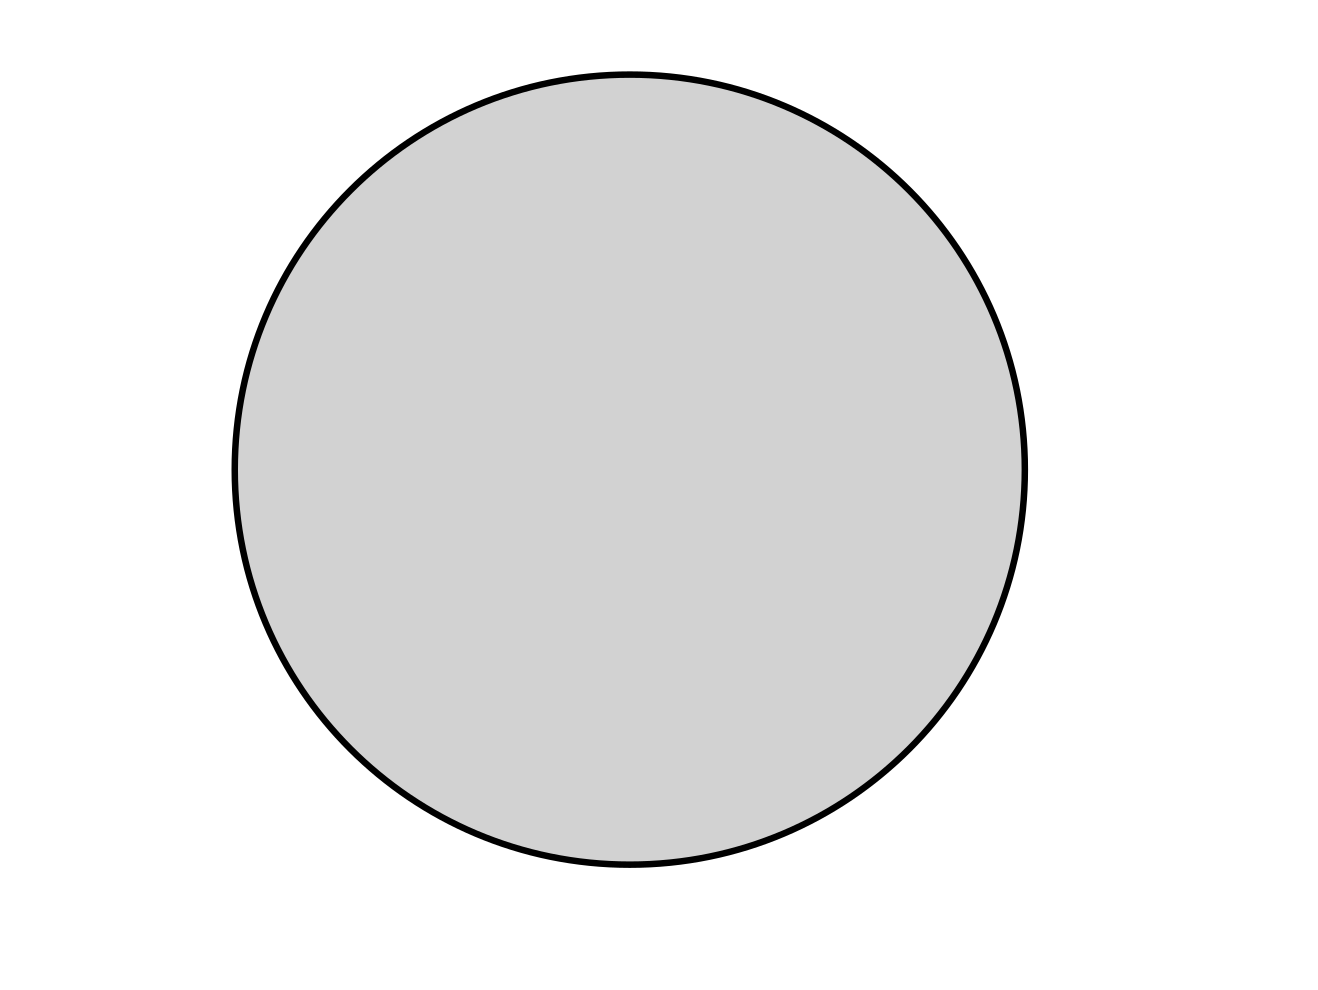
\includegraphics[scale = 0.15]{figure/圆}
\end{figure}

\begin{figure}[H]
	\centering
	\caption{圆周:$S^1$}
	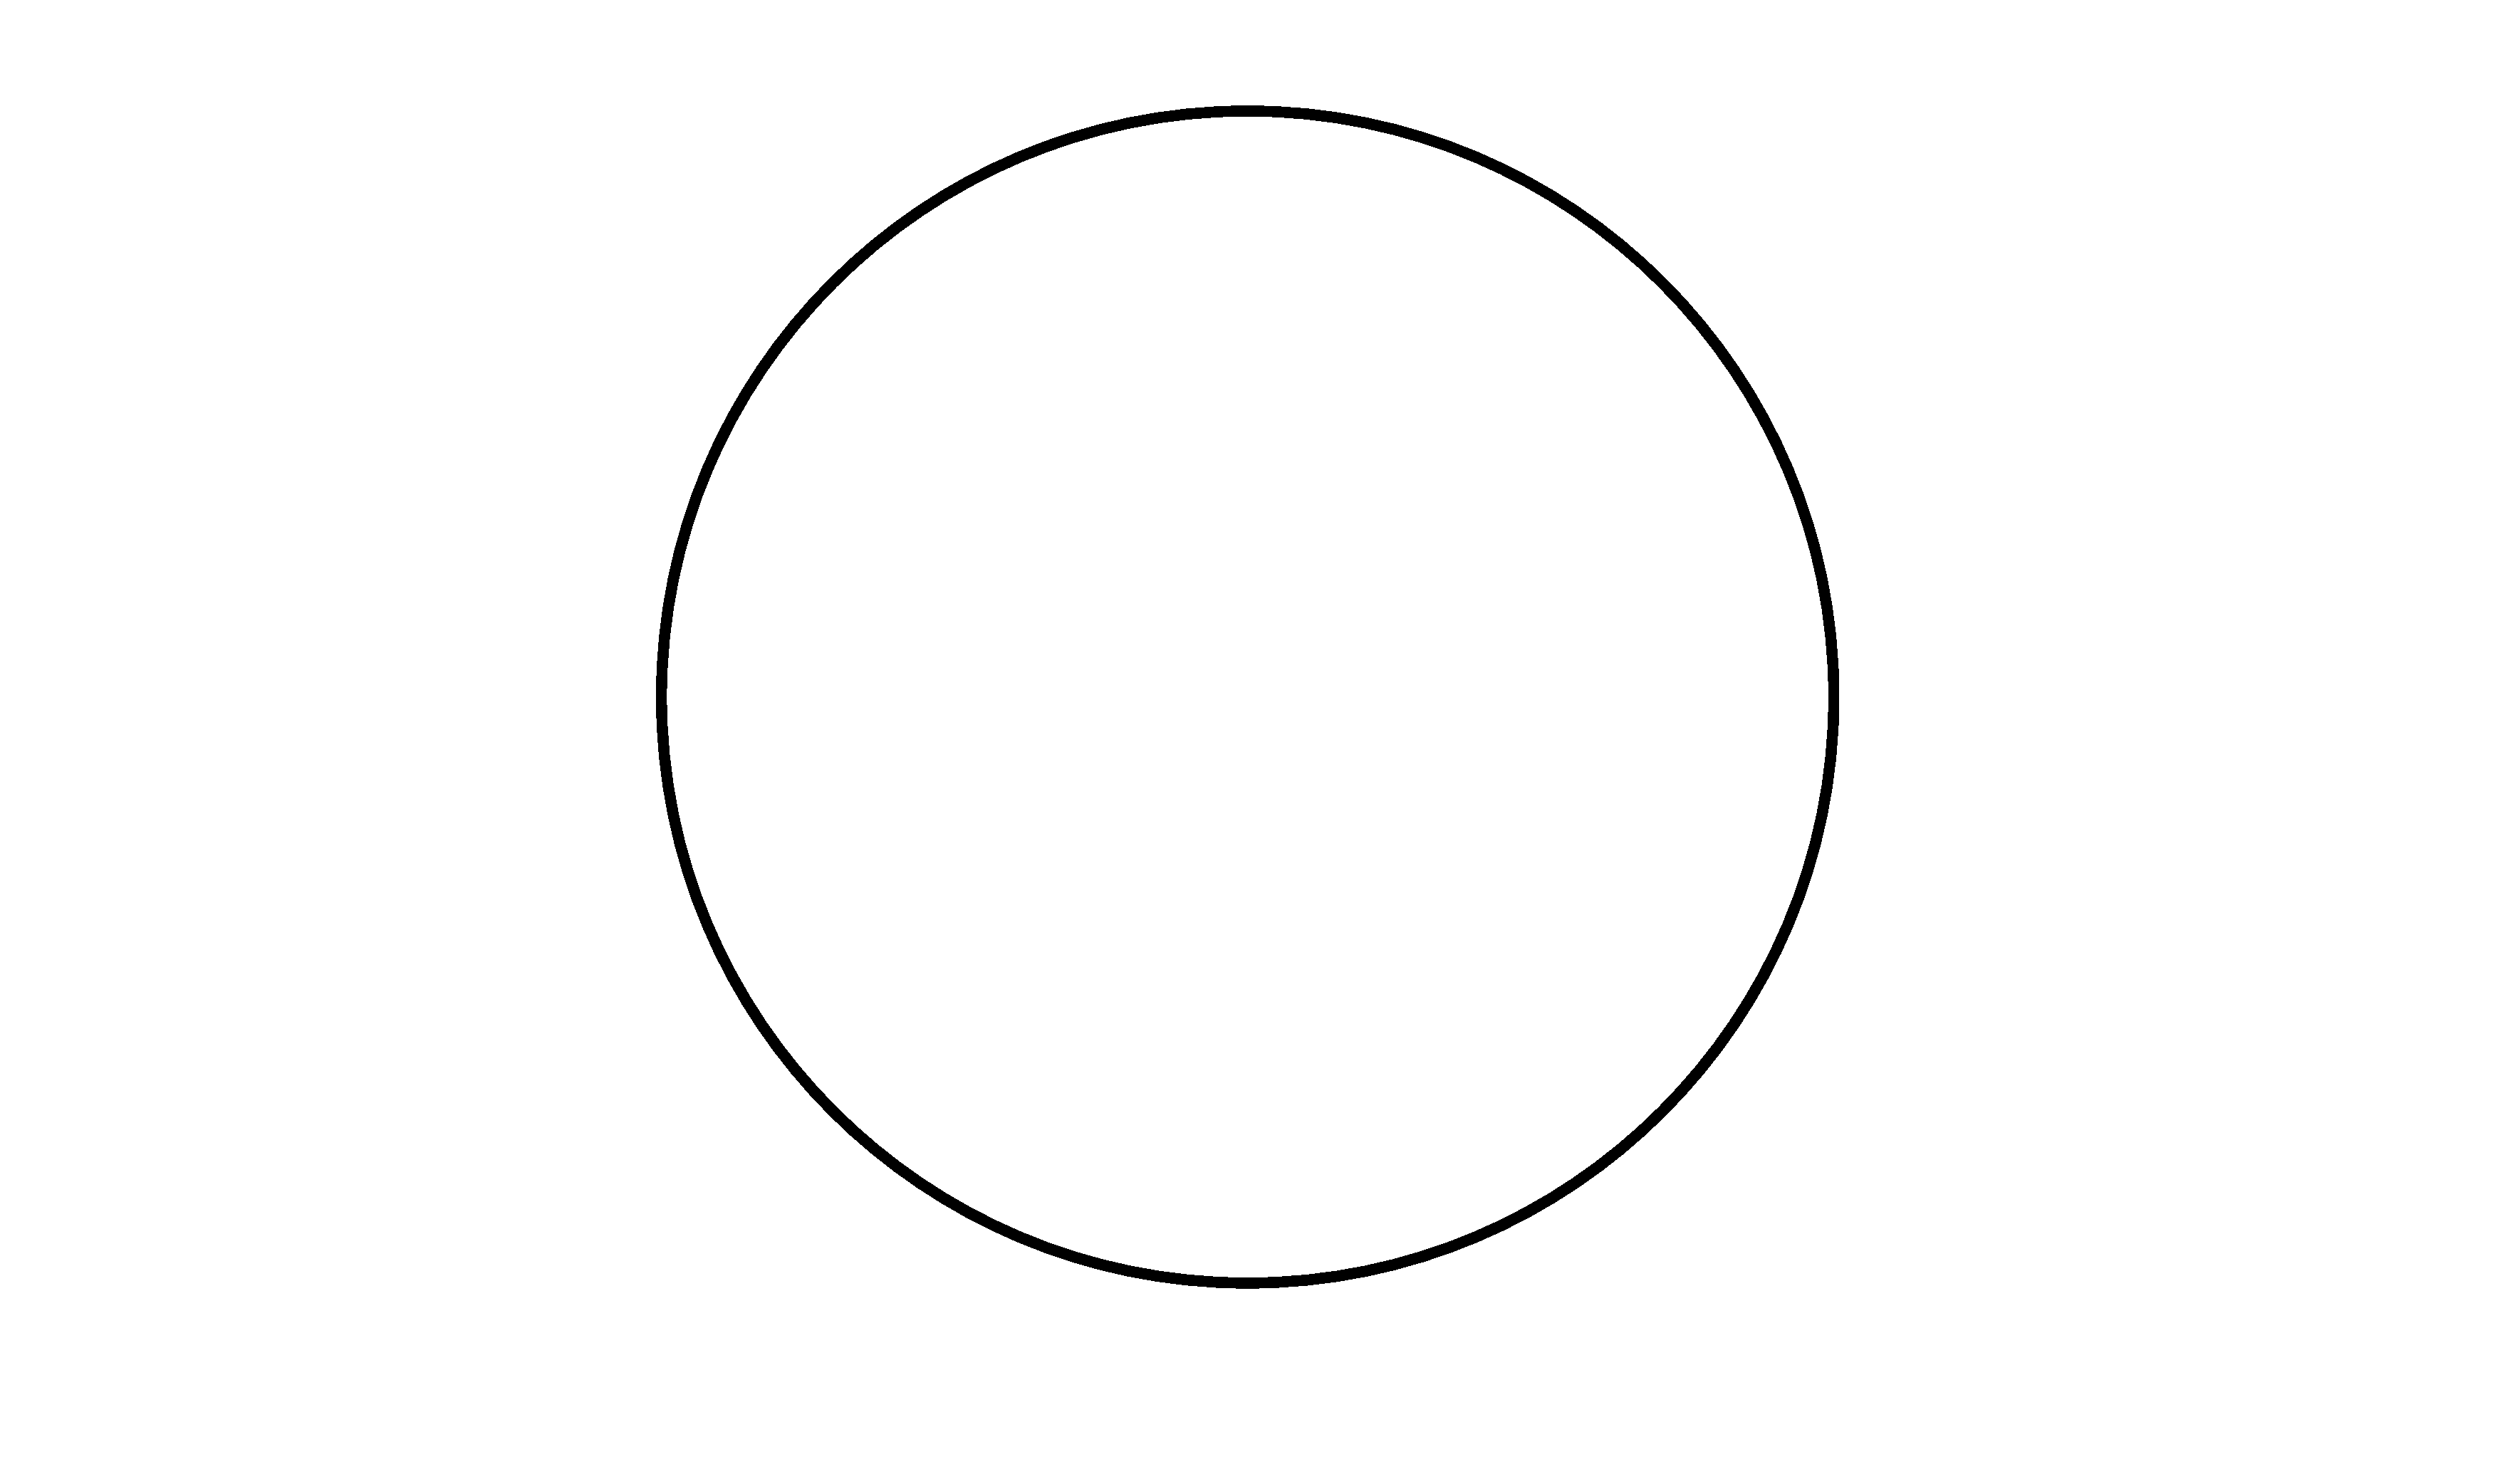
\includegraphics[scale = 0.15]{figure/圆周}
\end{figure}

\begin{figure}[H]
	\centering
	\caption{平环}
	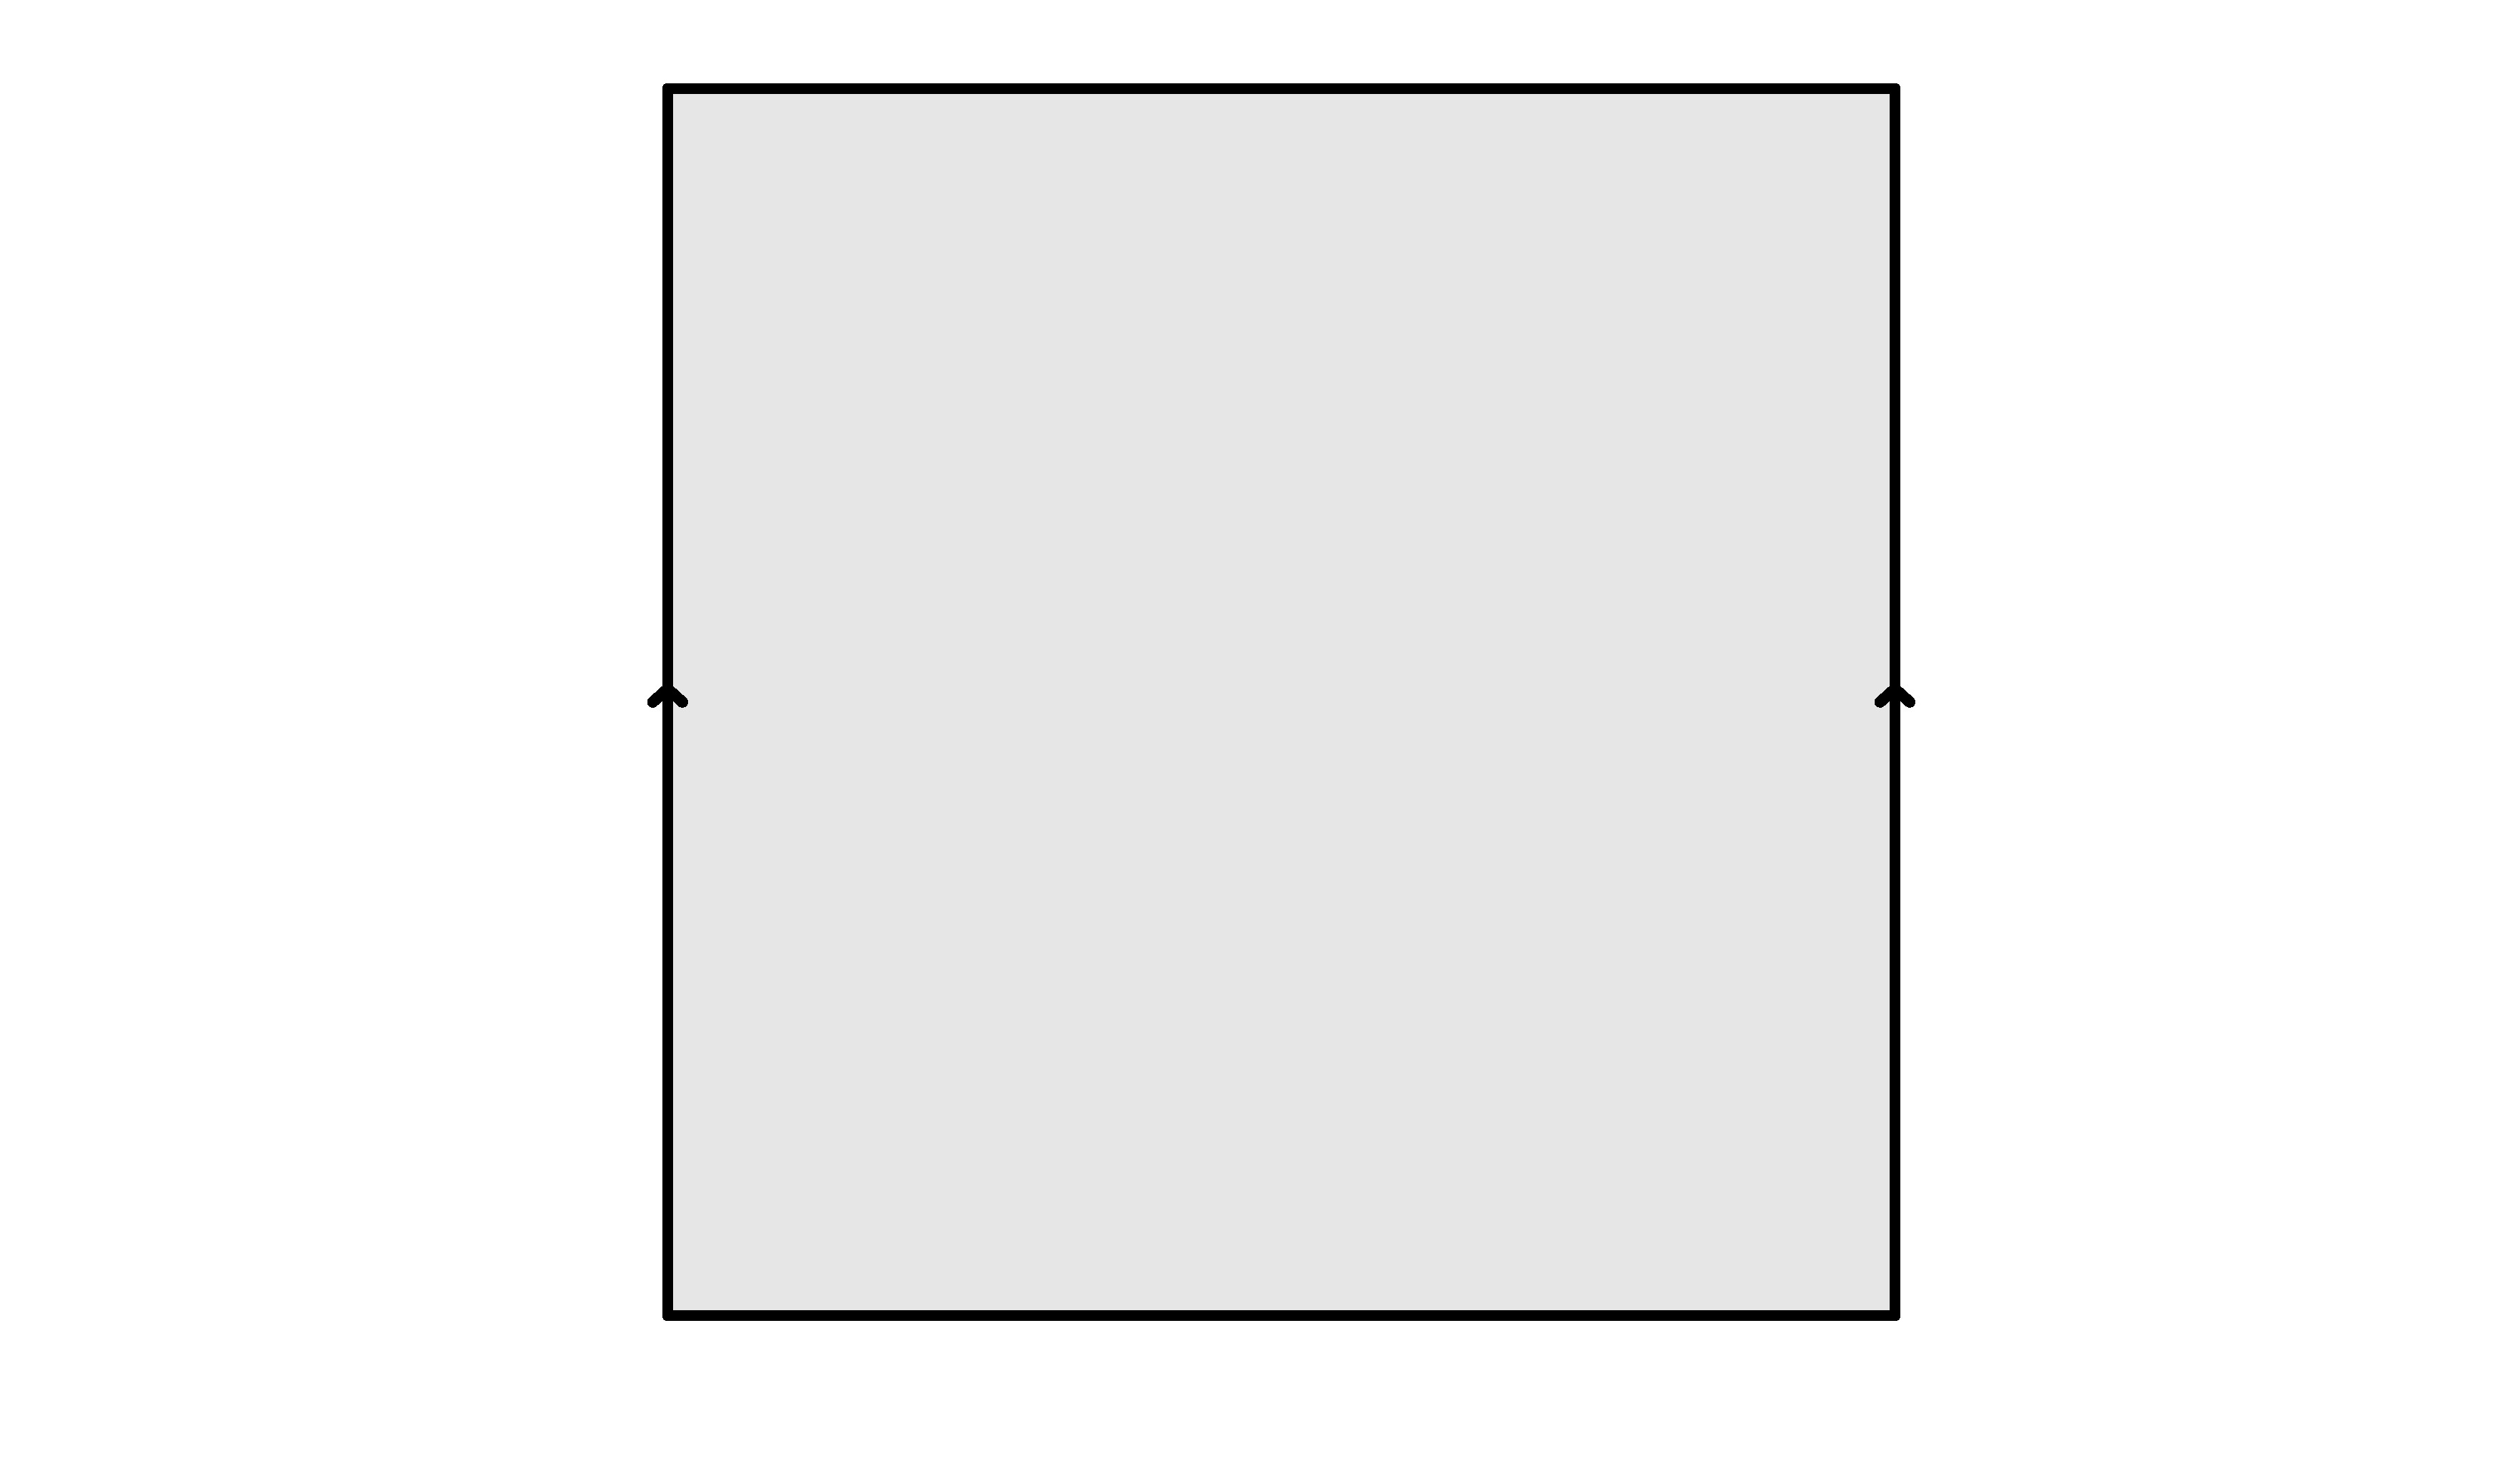
\includegraphics[scale = 0.15]{figure/平环}
\end{figure}

\begin{figure}[H]
	\centering
	\caption{Möbius带}
	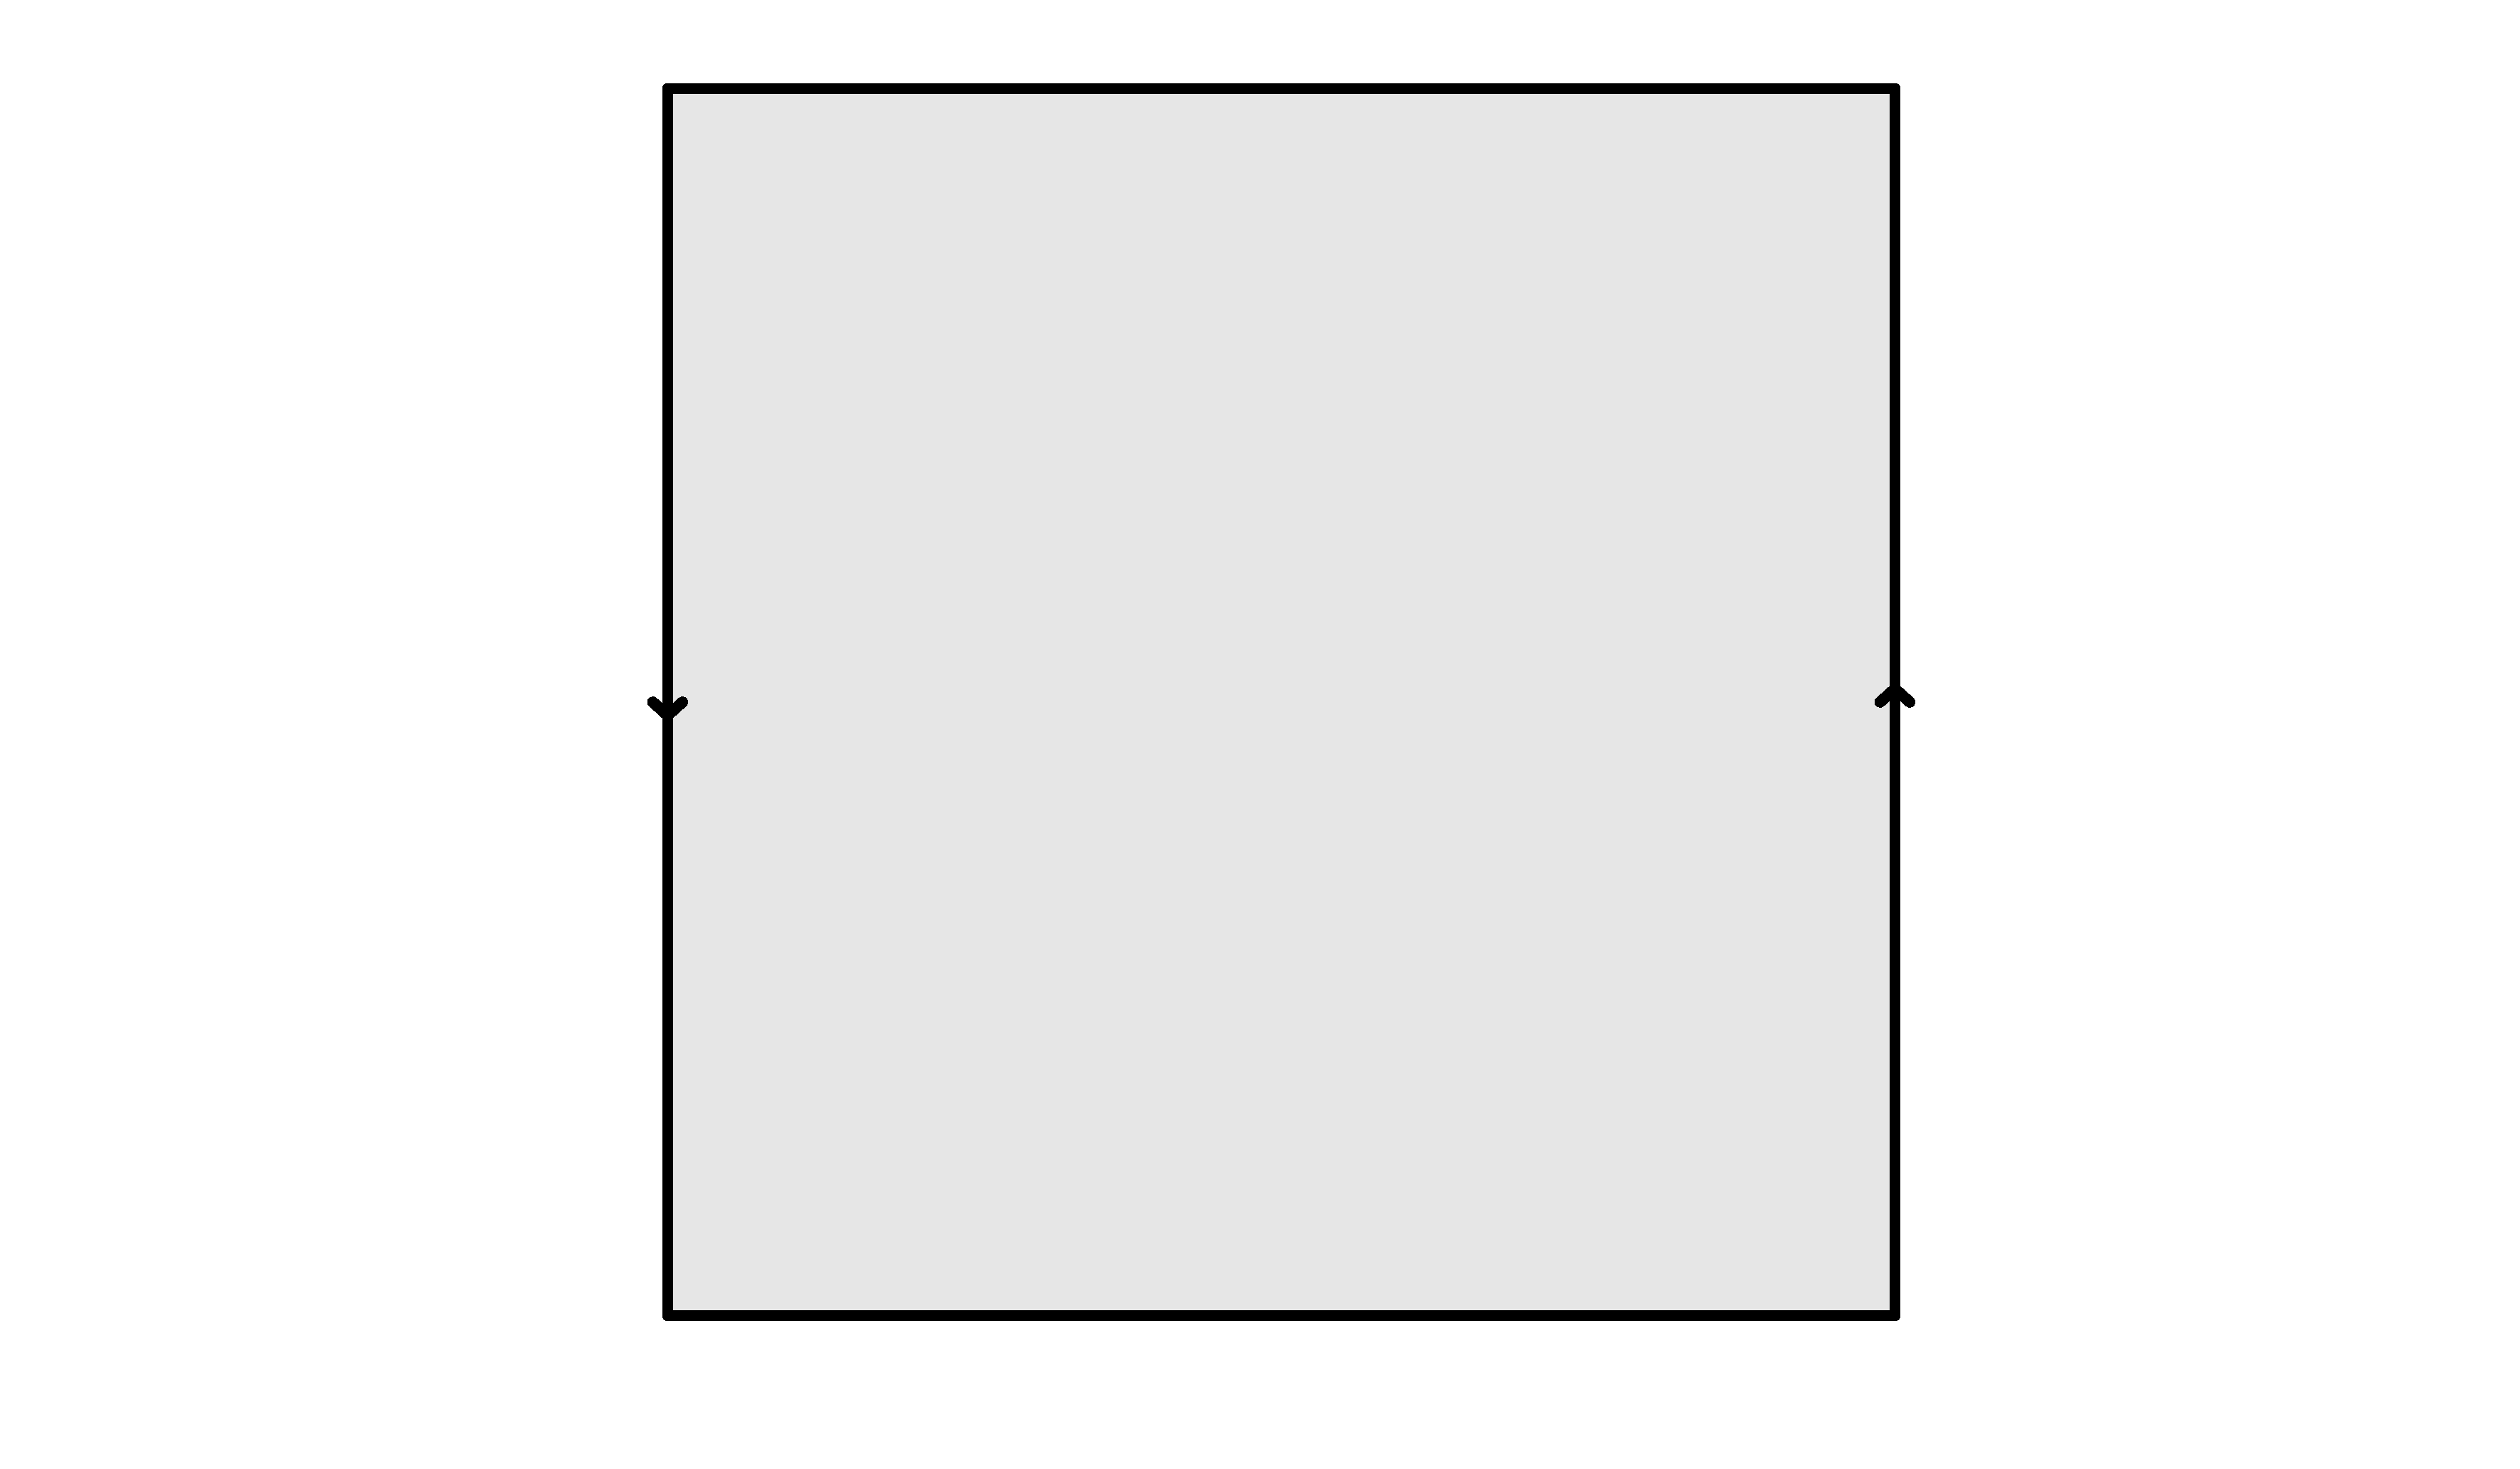
\includegraphics[scale = 0.15]{figure/Möbius带}
\end{figure}

\begin{figure}[H]
	\centering
	\caption{环面:$T^2$}
	\includegraphics[scale = 0.15]{figure/环面}
\end{figure}

\begin{figure}[H]
	\centering
	\caption{Klein瓶:$2P^2$}
	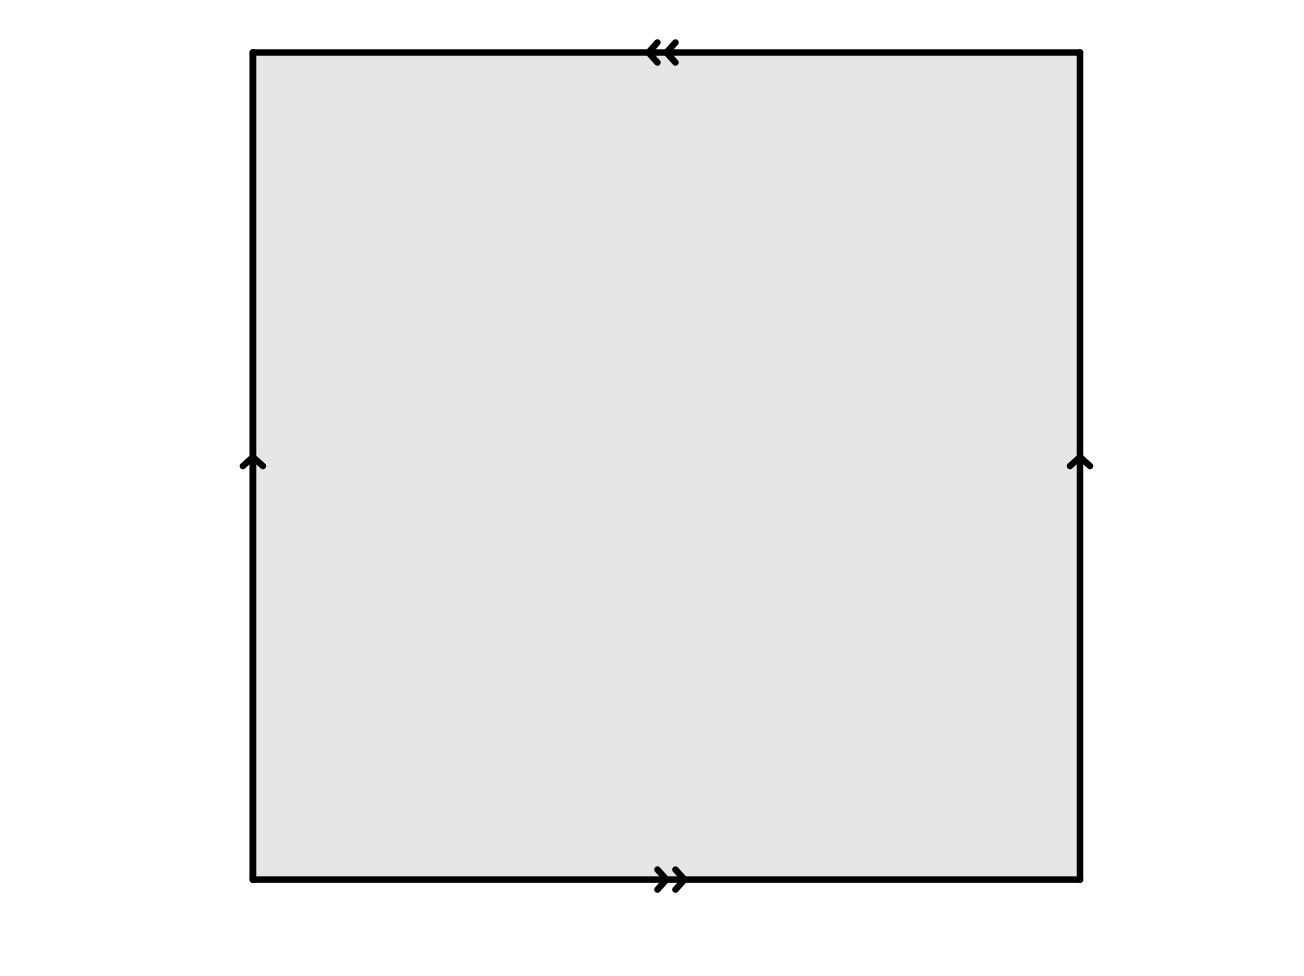
\includegraphics[scale = 0.15]{figure/Klein瓶}
\end{figure}

\begin{figure}[H]
	\centering
	\caption{射影平面:$P^2$}
	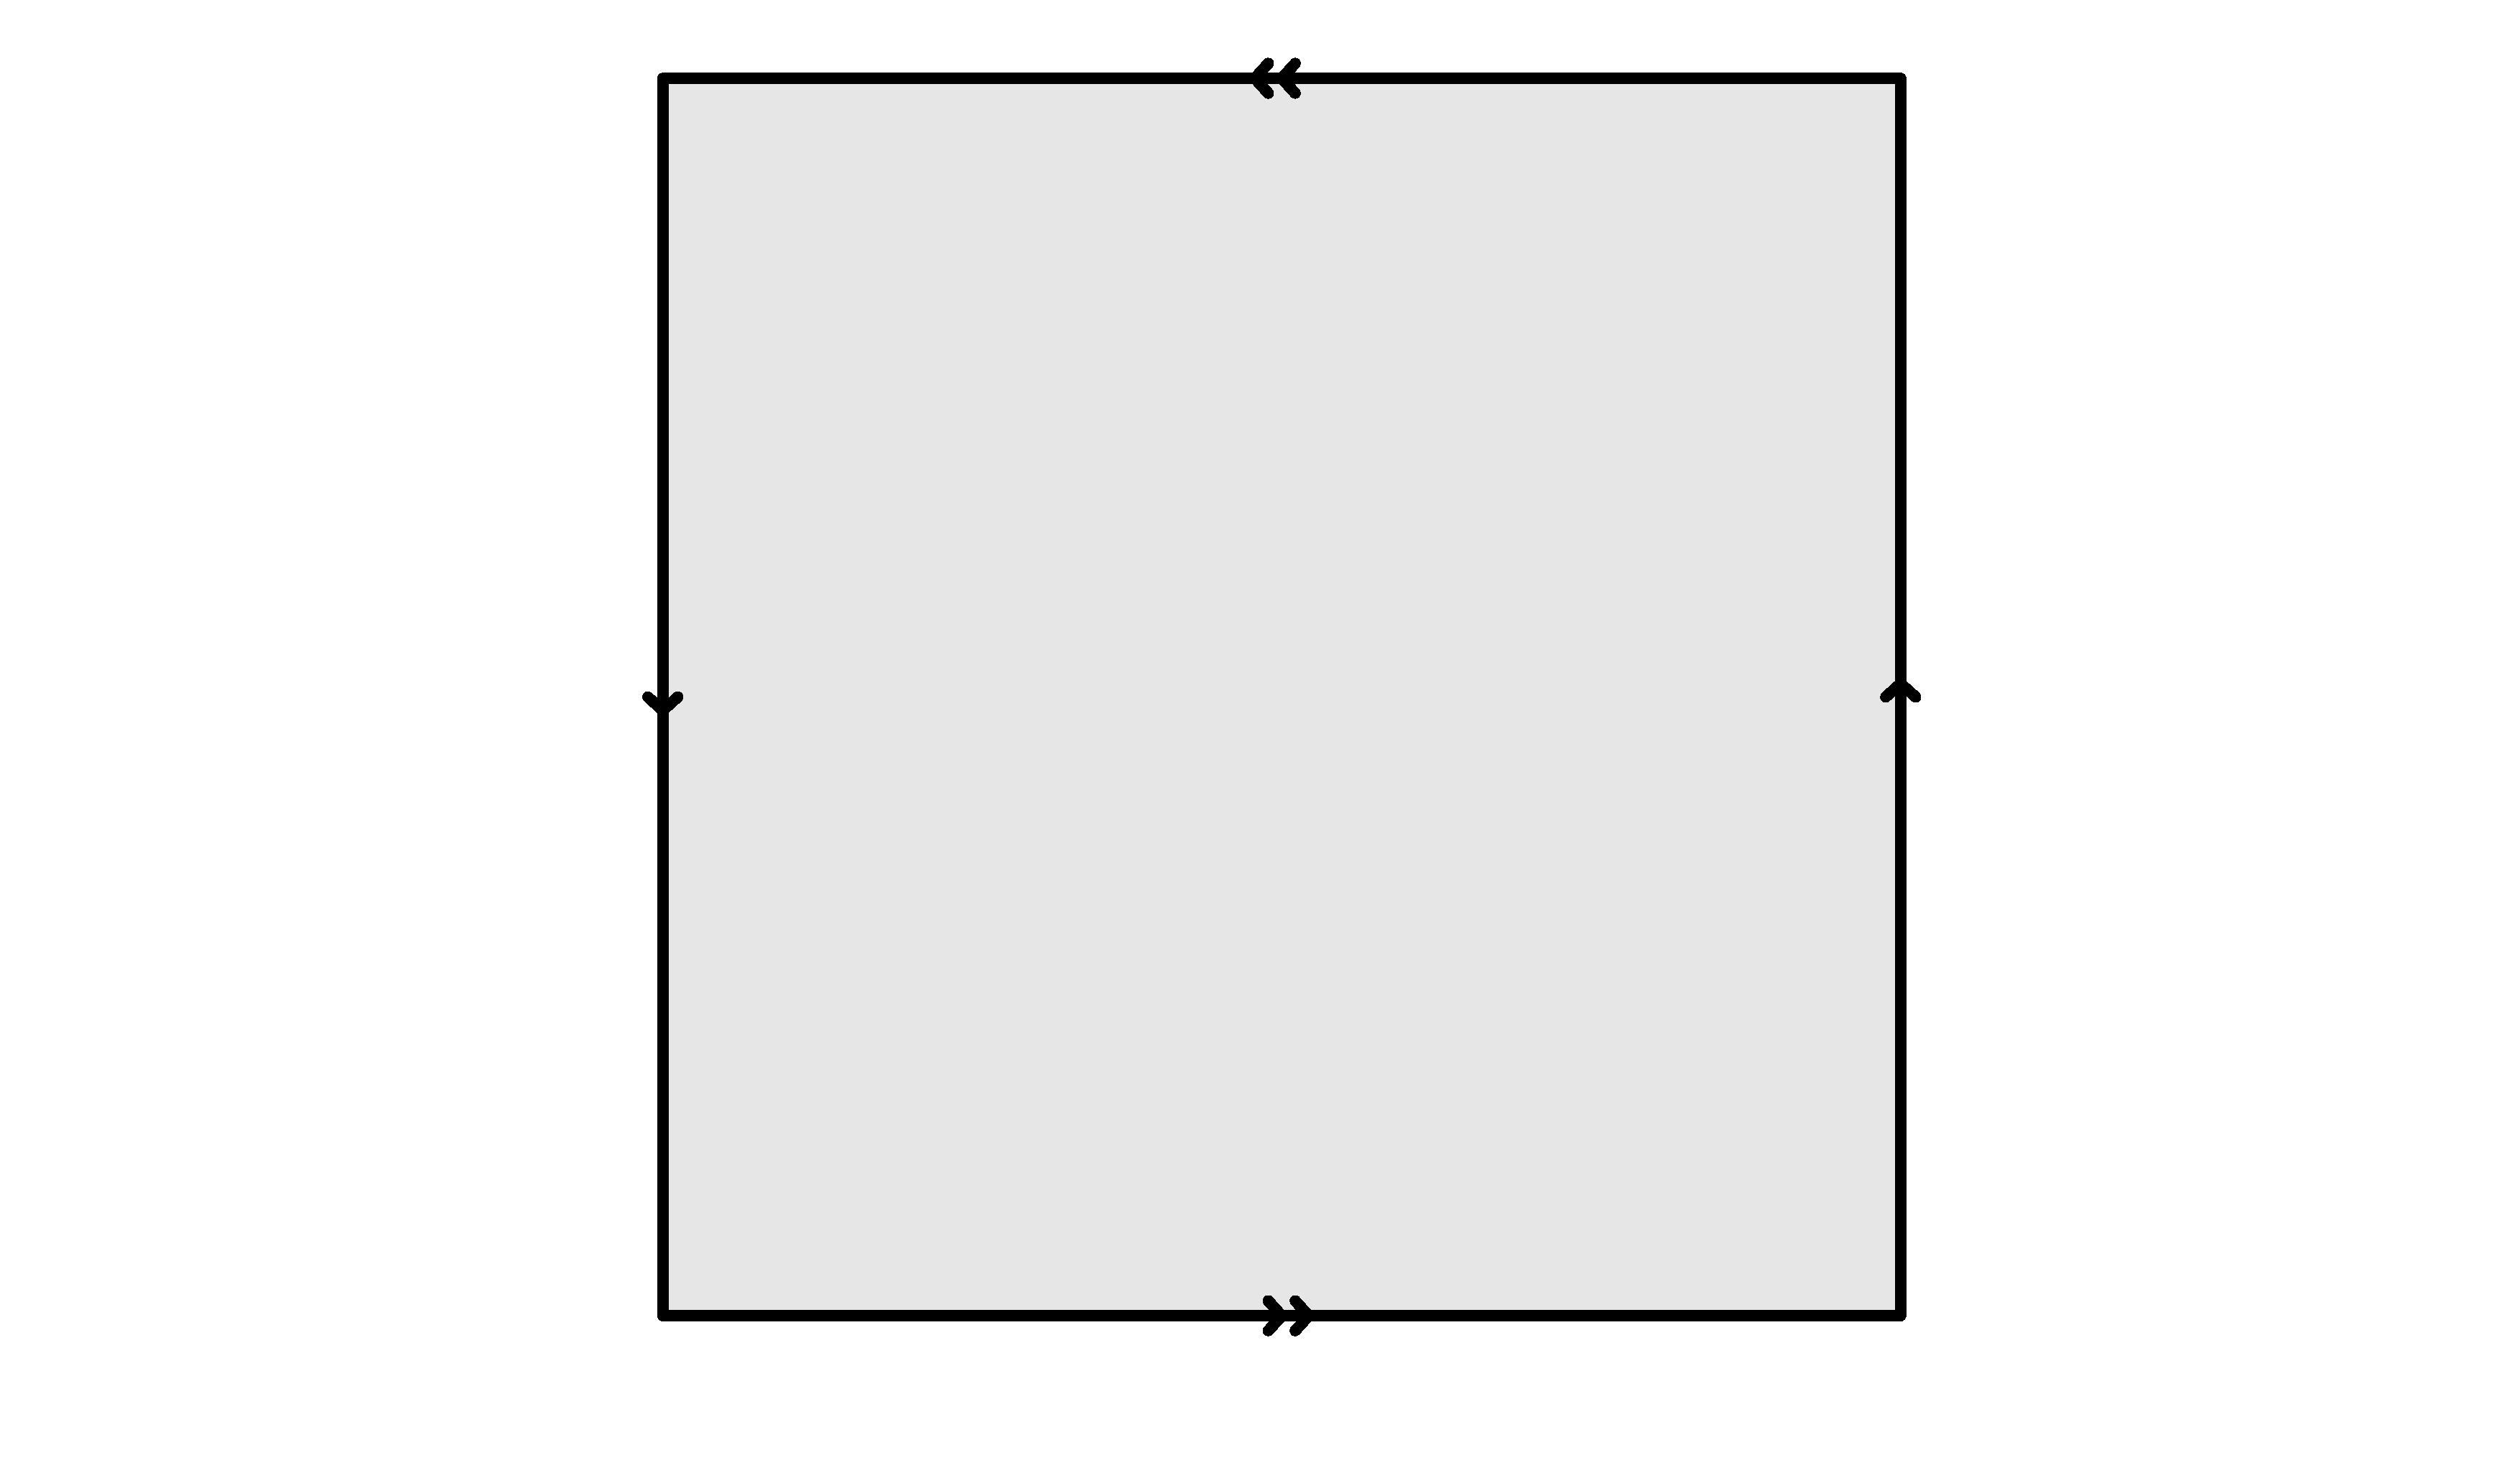
\includegraphics[scale = 0.15]{figure/射影平面}
\end{figure}

\begin{figure}[H]
	\centering
	\caption{环柄}
	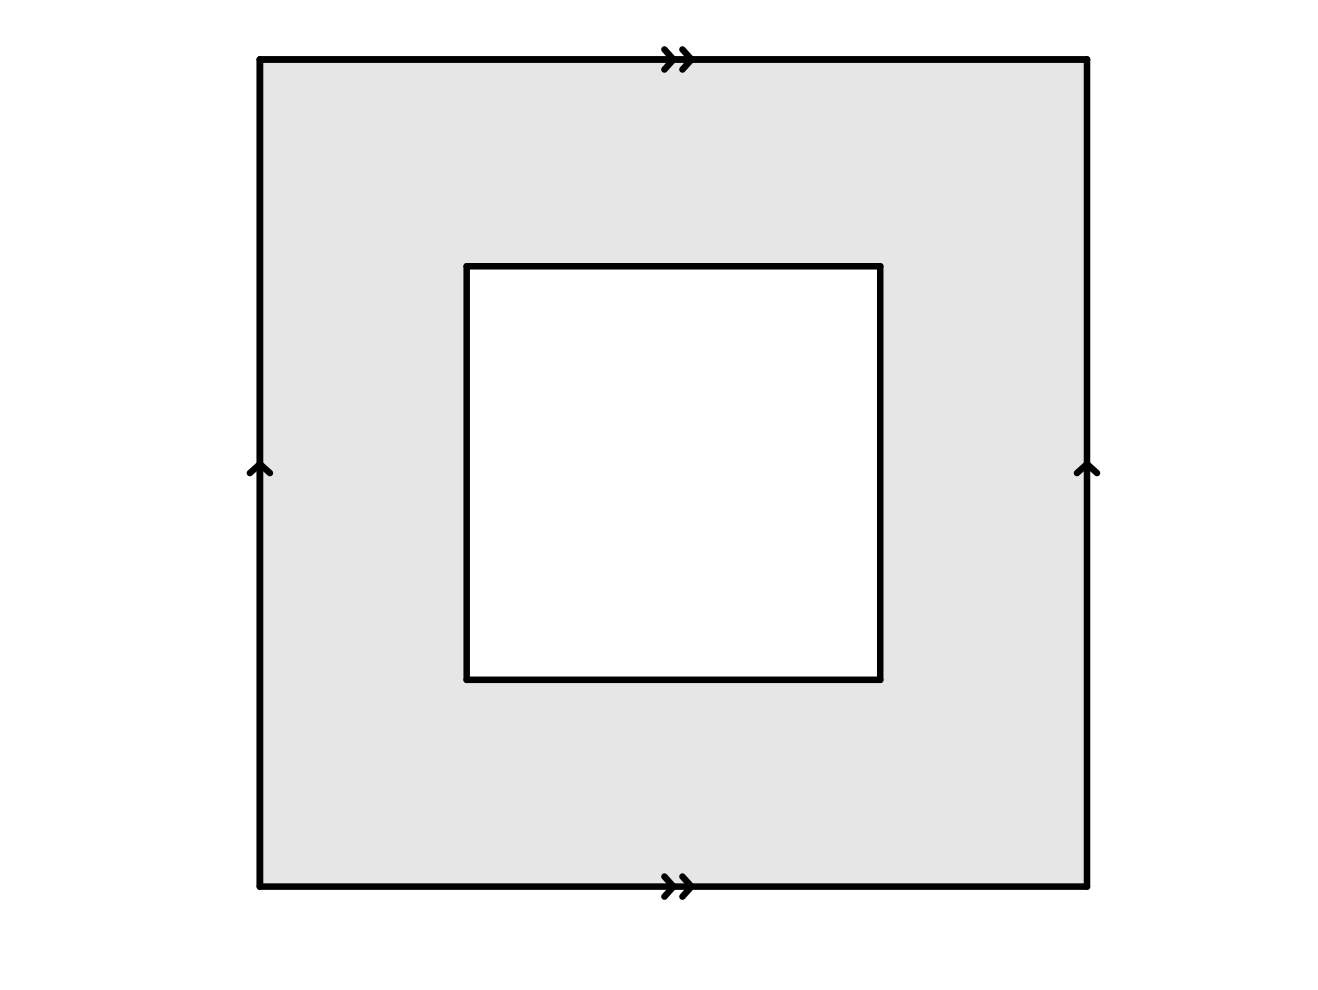
\includegraphics[scale = 0.15]{figure/环柄}
\end{figure}

\section{商空间与商映射}

\begin{definition}{商集}
	定义集合$X$关于等价关系$\sim$的商集为$X/\sim$。特别的,定义集合$X$关于子集$A$的商集为$X/ A=X/\overset{A}{\sim}$,其中$x_1\overset{A}{\sim} x_2\iff x_1=x_2\text{或}x_1,x_2\in A$。
\end{definition}

\begin{definition}{商拓扑}
	定义拓扑空间$(X,\tau)$关于等价关系$\sim$的商拓扑为
	$$
	\tilde{\tau}=\{ V\sub X/\sim :\pi^{-1}(V)\in \tau \}
	$$
	其中$\pi:X\to X/\sim$为自然映射。
\end{definition}

\begin{definition}{商空间}
	定义拓扑空间$(X,\tau)$关于等价关系$\sim$的商空间为$(X/\sim,\tilde{\tau})$。
\end{definition}

\begin{definition}{商映射}
	对于拓扑空间$X$与$Y$,称满映射$f:X\to Y$为商映射,如果对于任意$Y$的子集$B$,成立$B$为$Y$的开集$\iff f^{-1}(B)$为$X$的开集。
\end{definition}

\begin{theorem}{商映射的性质}
	\begin{enumerate}
		\item 自然映射$\pi:X\to X/\sim$为商映射。
		\item 对于拓扑空间$X,Y,Z$,如果$f:X\to Y$为商映射,那么映射$g:Y\to Z$连续$\iff$映射$g\circ f:X\to Z$连续。
		\item 如果$f:X\to Y$为商映射,那么$X/\overset{f}{\sim}\cong Y$,其中$x_1 \overset{f}{\sim} x_2\iff f(x_1)=f(x_2)$。
		\item 连续且满的开映射为商映射;连续且满的闭映射为商映射。
		\item 如果$X$为紧致空间,$Y$为Hausdorff空间,那么连续满映射$f:X\to Y$为商映射。
		\item 商映射的复合为商映射。
	\end{enumerate}
\end{theorem}

\section{拓扑流形与闭曲面}

\subsection{拓扑流形}

\begin{definition}{拓扑流形}
	称Hausdorff空间$X$为$n$维拓扑流形,如果对于任意点$x$,存在$x$的邻域$U$,使得成立或$U\cong E^n$,或$U\cong E^n_+$,其中$E^n_+=\{ (x_1,\cdots,x_n)\in E^n:x_n\ge 0 \}$。
\end{definition}

\begin{remark}
	\begin{enumerate}
		\item $E^n\not\cong E^n_+$
		\item $E^m\cong E^n\iff m=n$
		\item 拓扑流形为局部道路连通且局部紧致的$C_1$空间。
	\end{enumerate}
\end{remark}

\begin{definition}{内点}
	对于$n$维拓扑流形$X$,称点$x$为内点,如果存在$x$的开邻域$U$,使得成立$U\cong E^n$。
\end{definition}

\begin{definition}{边界点}
	对于$n$维拓扑流形$X$,称点$x$为边界点,如果对于任意$x$的开邻域$U$,成立$U\not\cong E^n$。
\end{definition}

\begin{definition}{内部}
	称拓扑流形$X$的内点全体为$X$的内部,记作$X^\circ$。
\end{definition}

\begin{definition}{边界}
	称拓扑流形$X$的边界点全体为$X$的边界,记作$\partial X$。
\end{definition}

\begin{proposition}
	$n$维拓扑流形的边界为无边界点的$n-1$维拓扑流形。
\end{proposition}

\subsection{闭曲面}

\begin{definition}{曲面}
	称二维流形为曲面。
\end{definition}

\begin{example}
	$E^2,D^2,S^2,T^2,P^2$以及平环、Möbius带、Klein瓶为曲面。
\end{example}

\begin{definition}{闭曲面}
	称无边界点的紧致连通曲面为闭曲面。
\end{definition}

\begin{example}
	\begin{enumerate}
		\item $S^2,T^2,P^2$以及Klein瓶为闭曲面。
		\item $E^2,D^2$以及平环、Möbius带不为闭曲面。
		\item 如果$\Gamma$为偶数边多边形,那么成对粘接边,可得闭曲面。
	\end{enumerate}
\end{example}

\begin{definition}{安环柄的球面}
	称安$n$个环柄的球面为亏格为$n$的可定向闭曲面,记作$nT^2$。
\end{definition}

\begin{definition}{安交叉帽的球面}
	称安$n$个Möbius带的球面为亏格为$n$的不可定向闭曲面,记作$nP^2$。
\end{definition}

\begin{definition}{闭曲面的标准表示}
	\begin{align*}
		& nT^2:a_1b_1a_1^{-1}b_1^{-1}a_2b_2a_2^{-1}b_2^{-1}\cdots a_nb_na_n^{-1}b_n^{-1}\\
		& mP^2:a_1a_1a_2a_2\cdots a_ma_m
	\end{align*}
\end{definition}

\begin{theorem}{闭曲面分类定理}
	\begin{enumerate}
		\item 闭曲面或为$nT^2$,或为$mP^2$,其中$n\in\N$且$m\in\N^*$。
		\item $\{ nT^2:n\in\N \}\cap \{ mP^2:m\in\N^* \}=\varnothing$
		\item $m=n\iff mT^2=nT^2=\iff mP^2=nP^2$
		\item 如果闭曲面的多边形表示存在同向边时,该闭曲面为$(l/2-k+1)P^2$;否则为$((l/2-k+1)/2)T^2$。其中$l$为边数,$k$为顶点类数。
	\end{enumerate}
\end{theorem}

\begin{definition}{连通与}
	将两个闭曲面挖去一个圆,然后将洞口对接,所得闭曲面称为原来两个闭曲面的连通与,记作$M\# N$。
\end{definition}

\begin{theorem}{闭曲面的连通与}
	\begin{enumerate}
		\item $mT^2\# nT^2=(m+n)T^2$
		\item $mP^2\# nP^2=(m+n)P^2$
		\item $mT^2\# nP^2=(2m+n)P^2$
	\end{enumerate}
\end{theorem}

\begin{lstlisting}[language = Matlab, caption = {闭曲面分类定理主函数}]
	clear; clc
	
	% 输入闭曲面的多边形表示字符串
	% 例如输入:ab-1a-1cdcbd
	string = input('请输入字符串:', 's');
	
	% 调用函数
	[type, edgeNumber, nodeNumber] = closedSurfaceType(string);
	
	% 输出
	fprintf('边数为: %d\n', edgeNumber)
	fprintf('节点类数为: %d\n', nodeNumber)
	fprintf('闭曲面类型为: %s\n', type)
	
\end{lstlisting}

\begin{lstlisting}[language = Matlab, caption = {闭曲面类型函数}]
	function [type, edgeNumber, nodeNumber] = closedSurfaceType(string)
	    
	    % 名称:闭曲面类型
	    % 输入:
	    %      string:字符串
	    % 输出:
	    %      type:闭曲面类型
	    %      edgeNumber:边数
	    %      nodeNumber:节点类数
	    % 说明:
	    %      输入为字符串,类型为:
	    %      一个字母+其他类型(或没有)+一个字母+其他类型(或没有)+...
	    %      相同字母仅输入且输入两次
	    %      例如:ab^-1a0cdcbd
	
	    %% 函数
	
	    % 定义多边形表示矩阵
	    polygonsRepresentMatrice = stringToMatrix(string);
	
	    % 定义边数
	    edgeNumber = size(polygonsRepresentMatrice, 2);
	
	    % 判断是否由同向对
	    sameDirectionPairs = 0;
	    for i = 1: edgeNumber - 1
	        for j = i + 1: edgeNumber
	            if all(polygonsRepresentMatrice(:, i) == polygonsRepresentMatrice(:, j))
	                sameDirectionPairs = 1;
	            end
	        end
	    end
	
	    % 计算节点类数
	    nodeNumber = nodeClass(string);
	
	    % 计算闭曲面类型
	    if sameDirectionPairs == 1
	        n = (edgeNumber - 2 * nodeNumber + 2) / 2;
	        type = [num2str(n), 'P^2'];
	    else
	        n = (edgeNumber - 2 * nodeNumber + 2) / 4;
	        type = [num2str(n), 'T^2'];
	    end
	
	end
	
\end{lstlisting}

\begin{lstlisting}[language = Matlab, caption = {节点类函数}]
	function [equivalentClassNumber, equivalentClassMatrix] = nodeClass(string)
	    
	    % 名称:节点类
	    % 输入:
	    %      string:字符串
	    % 输出:
	    %      equivalentClassNumber:闭曲面的顶点类数
	    %      equivalentClassMatrix:闭曲面的顶点类矩阵
	    % 说明:
	    %      输入为字符串,类型为:
	    %      一个字母+其他类型(或没有)+一个字母+其他类型(或没有)+...
	    %      相同字母仅输入且输入两次
	    %      例如:ab^-1a0cdcbd
	
	    %% 准备
	
	    % 定义多边形表示矩阵
	    polygonsRepresentMatrice = stringToMatrix(string);
	
	    % 定义节点数量
	    nodeNumber = size(polygonsRepresentMatrice, 2);
	    
	    % 定义节点矩阵
	    nodeMatrix = [polygonsRepresentMatrice' zeros(nodeNumber, 2)];
	    for n = 1: nodeNumber
	        if nodeMatrix(n, 2) == 0
	            nodeMatrix(n, 3: 4) = [n mod(n-2, nodeNumber) + 1];
	        else
	            nodeMatrix(n, 3: 4) = [mod(n-2, nodeNumber) + 1 n];
	        end
	    end
	    
	    %% 计算顶点类数和顶点类矩阵
	    
	    equivalentClassNumber = 0;                             % 初始化等价类数目
	    allNode = 1: nodeNumber;                               % 全部节点
	    selectedNode = zeros(1, nodeNumber);                   % 初始化已选节点
	    selectedNodeNumber = 0;                                % 初始化已选节点数目
	    equivalentClassMatrix = [];                            % 初始化等价类矩阵
	    
	    while selectedNodeNumber < nodeNumber % 设置while循环,直至选取全部节点
	    
	        unselectedNode = setdiff(allNode, selectedNode); % 重置未选节点
	        firstNode = unselectedNode(1);                   % 首节点
	        currentSelectedNode = zeros(1, nodeNumber);      % 初始化已选节点
	        currentSelectedNodeNumber = 0;                   % 初始化已选节点数目
	    
	        for n = 1: nodeNumber % 循环寻找首节点所在边和方向
	            judge = 1;
	            for direc = 3: 4 % 3表示前节点,4表示后节点
	                if nodeMatrix(n, direc) == firstNode
	                    firstedge = n;                % 首边
	                    firstType = nodeMatrix(n, 1); % 首边类型
	                    firstDirection = direc;       % 首节点位于首边的方向
	                    judge = 0;
	                    break
	                end
	            end
	            if judge == 0
	                break
	            end
	        end
	        
	        currentNode = 0;                   % 初始化迭代节点
	        currentedge = firstedge;           % 初始化迭代边
	        currentType = firstType;           % 初始化迭代边类型
	        currentDirection = firstDirection; % 初始化迭代节点位于迭代边的方向
	    
	        while firstNode ~= currentNode % 直至所选节点围成圈为止
	            
	            % 寻找同类型的边
	            for n = 1: nodeNumber
	                if n ~= currentedge && nodeMatrix(n, 1) == currentType
	                    sameTypeedge = n; % 设置同类型的边
	                    break
	                end
	            end
	            currentNode = nodeMatrix(sameTypeedge, currentDirection); % 更新迭代节点
	            
	            % 寻找迭代节点所在的其他边
	            for direc = 3: 4 % 3表示前节点,4表示后节点
	                if nodeMatrix(mod(sameTypeedge-2, nodeNumber)+1, direc) == currentNode % 如果迭代节点为前边的节点
	                    currentedge = mod(sameTypeedge - 2, nodeNumber) + 1; % 更新迭代边
	                    currentType = nodeMatrix(currentedge, 1);            % 更新迭代边类型
	                    currentDirection = direc;                            % 更新迭代节点位于迭代边的方向
	                end
	            end
	            for direc = 3: 4 % 3表示前节点,4表示后节点
	                if nodeMatrix(mod(sameTypeedge, nodeNumber)+1, direc) == currentNode % 如果迭代节点为后边的节点
	                    currentedge = mod(sameTypeedge, nodeNumber) + 1; % % 更新迭代边
	                    currentType = nodeMatrix(currentedge, 1);        % 更新迭代边类型
	                    currentDirection = direc;                        % 更新迭代节点位于迭代边的方向
	                end 
	            end
	    
	            currentSelectedNodeNumber = currentSelectedNodeNumber + 1;    % 更新迭代已选节点数目
	            selectedNodeNumber = selectedNodeNumber + 1;                  % 更新已选节点数目
	            currentSelectedNode(currentSelectedNodeNumber) = currentNode; % 更新迭代已选节点
	            selectedNode(selectedNodeNumber) = currentNode;               % 更新已选节点
	             
	        end
	    
	        for n = 1: nodeNumber % 修改已选节点矩阵的呈现
	            if n ~= nodeNumber
	                if currentSelectedNode(n + 1) == 0
	                    currentSelectedNode = [currentSelectedNode(n) currentSelectedNode];
	                    currentSelectedNode(n + 1) = [];
	                    break
	                end
	            else
	                currentSelectedNode = [currentSelectedNode(nodeNumber) currentSelectedNode];
	                currentSelectedNode(nodeNumber + 1) = [];
	            end
	        end
	    
	        equivalentClassNumber = equivalentClassNumber + 1;                     % 更新等价类数目
	        equivalentClassMatrix(equivalentClassNumber, :) = currentSelectedNode; % 更新等价类矩阵
	          
	    end
	    
	    % 去除等价类矩阵的零列
	    for n = nodeNumber: -1: 1
	        if sum(equivalentClassMatrix(:, n)) == 0
	            equivalentClassMatrix(:, n) = [];
	        else
	            break
	        end
	    end
	
	end
	
\end{lstlisting}

\begin{lstlisting}[language = Matlab, caption = {字符串转为矩阵函数}]
	function matrix = stringToMatrix(string)
	    
	    % 名称:字符串转为矩阵
	    % 输入:
	    %      string:字符串
	    % 输出:
	    %      matrix:矩阵
	    % 说明:
	    %      输入为字符串,类型为:
	    %      一个字母+其他类型(或没有)+一个字母+其他类型(或没有)+...
	    %      相同字母仅输入且输入两次
	    %      例如:ab^-1a0cdcbd
	    %
	    %      输出为2行矩阵
	    %      第一行代表边类型
	    %      第二行代表边方向
	    %      例如输入:
	    %                a b^{-1} a^{-1} c d c b d
	    %      输出矩阵为:
	    %                1   2      1    3 4 3 2 4
	    %                0   1      1    0 0 0 0 0
	
	
	    %% 函数
	    % 使用正则表达式提取字母
	    letterArray = regexp(string, '[a-zA-Z]', 'match');
	    
	    % 创建一个结构体来存储字母和对应的值
	    letterStruct = struct();
	    
	    % 初始化一个计数器
	    count = 1;
	    % 遍历字母数组
	    for n = 1: length(letterArray)
	        % 获取当前字母
	        letter = letterArray{n};  
	        % 检查字母是否已经在结构体中
	        if isfield(letterStruct, letter)
	            % 字母已存在,不需要重复存储
	            continue;
	        end
	        % 将字母存储在结构体中,并分配一个唯一的值
	        letterStruct.(letter) = count;  
	        % 增加计数器
	        count = count + 1;
	    end
	    
	    % 初始化矩阵
	    matrix = zeros(2, length(string));
	    % 转化为矩阵
	    for n = 1: length(string)
	        if isletter(string(n))
	            matrix(1, n) = letterStruct.(string(n));
	            if n < length(string) && ~isletter(string(n+1))
	                matrix(2, n) = 1;
	            end
	        end
	    end
	    % 找到全是0的列的索引
	    zeroColumns = all(matrix == 0, 1);
	    % 删除全是0的列
	    matrix = matrix(:, ~zeroColumns);
	
	end
	
\end{lstlisting}

\chapter{基本群}

\section{同伦映射}

\subsection{同伦}

\begin{definition}{同伦}
	对于拓扑空间$X$与$Y$,称连续映射$f,g:X\to Y$同伦,并记做$f\overset{H}{\simeq}g$,或$H:f\simeq g$,如果存在连续映射$H:X\times I \to Y$,使得成立%
	$$
	H(x,0)=f(x),\qquad
	H(x,1)=g(x),\qquad
	x\in X
	$$
	同伦关系为等价关系,记$X\to Y$上的连续映射在同伦关系下的等价类为$[X,Y]$。
\end{definition}

\begin{example}
	对于拓扑空间$X$,以及凸集$Y\sub E^n$,定义连续映射$f,g:X\to Y$的直线同伦为
	\begin{align*}
		H:\begin{aligned}[t]
			X\times I &\longrightarrow Y\\
			(x,t) &\longmapsto (1-t)f(x)+tg(x)
		\end{aligned}
	\end{align*}
\end{example}

\begin{example}
	对于拓扑空间$X$,如果连续映射$f,g:X\to S^n$成立对于任意$x\in X$,成立$f(x)+g(x)\ne0$,那么$f$与$g$间的同伦为
	\begin{align*}
		H:\begin{aligned}[t]
			X\times I &\longrightarrow S^n\\
			(x,t) &\longmapsto \frac{(1-t)f(x)+tg(x)}{\|(1-t)f(x)+tg(x)\|}
		\end{aligned}
	\end{align*}
\end{example}

\begin{example}
	对于拓扑空间$X$,如果连续映射$f,g:X\to S^1$成立对于任意$x\in X$,成立$f(x)+g(x)=0$,那么$f$与$g$间的同伦为
	\begin{align*}
		H:\begin{aligned}[t]
			X\times I &\longrightarrow S^1\\
			(x,t) &\longmapsto \frac{\mathrm{e}^{it\pi}}{f(x)}
			\end{aligned}
	\end{align*}
\end{example}

\begin{proposition}{同伦的复合}
	如果$f_0\simeq f_1:X\to Y$,且$g_0\simeq g_1:Y\to Z$,那么$g_0\circ f_0\simeq g_1\circ f_1:X\to Z$。
\end{proposition}

\subsection{相对同伦}

\begin{definition}{相对同伦}
	对于拓扑空间$X$与$Y$,称连续映射$f,g:X\to Y$相对于$A\sub X$同伦,并记做$f\overset{H}{\simeq}g\text{ rel}A$,或$H:f\simeq g\text{ rel}A$,如果存在连续映射$H:X\times I \to Y$,使得成立%
	\begin{align*}
		& H(x,0)=f(x), &&
		H(x,1)=g(x), &&
		x\in X\\
		& H(a,t)=f(a), &&
		H(a,t)=g(a), &&
		(a,t)\in A\times I
	\end{align*}
	相对于$A$的同伦关系为等价关系。
\end{definition}

\begin{proposition}{相对同伦的复合}
	如果$f_0\simeq f_1\text{ rel}A$,且$g_0\simeq g_1\text{ rel}A$,那么$g_0\circ f_0\simeq g_1\circ f_1\text{ rel}A$。
\end{proposition}

\section{基本群}

\subsection{定端同伦}

\begin{definition}{定端同伦}
	称道路$a,b: I \to X$定端同伦,并记做$a\underset{\dot{}}{\simeq}b$,如果存在连续映射$H: I \times I \to X$,使得成立
	\begin{align*}
		&H(s,0)=a(s),&&
		H(s,1)=b(s),&&
		s\in I \\
		&H(0,t)=a(0)=b(0),&&
		H(1,t)=a(1)=b(1),&& 
		t\in I 
	\end{align*}
	定端同伦关系为等价关系。
\end{definition}

\begin{proposition}{定端同伦的性质}
	\begin{enumerate}
		\item 如果$a \underset{\dot{}}{\simeq} b$,那么$\overline{a}\underset{\dot{}}{\simeq}\overline{b}$。
		\item 如果$a_1 \underset{\dot{}}{\simeq} b_1$,且$a_2 \underset{\dot{}}{\simeq} b_2$,同时$a_1(1)=a_2(0)$,那么$b_1(1)=b_2(0)$,且$a_1a_2\underset{\dot{}}{\simeq}b_1b_2$。
		\item 如果$a(1)=b(0)$,且$b(1)=c(0)$,那么$(ab)c \underset{\dot{}}{\simeq} a(b c)$。
		\item 对于连续映射$f:X\to Y$,道路$a,b: I \to X$,如果$a \underset{\dot{}}{\simeq} b$,那么$f\circ a \underset{\dot{}}{\simeq} f\circ b$。
		\item 对于连续映射$f:X\to Y$,道路$a,b: I \to X$,如果$a(1)=b(0)$,那么$(f\circ a)(1)=(f\circ b)(0)$,且$(f\circ a)(f\circ b)=f\circ(ab)$。
		\item 对于连续映射$f:X\to Y$,道路$a: I \to X$,成立$\overline{f\circ a}=f\circ\overline{a}$。
	\end{enumerate}
\end{proposition}

\subsection{道路类}

\begin{definition}{道路类}
	称道路$a: I \to X$在定端同伦下的等价类为道路类,记作$[a]$。拓扑空间$X$的道路类全体记作$[X]$。
\end{definition}

\begin{definition}{道路类的逆}
	定义拓扑空间$X$上的道路类$\alpha$的逆为$\alpha^{-1}=[\overline{a}]$,其中$a\in\alpha$。
\end{definition}

\begin{definition}{道路类的积}
	如果$\alpha(1)=\beta(0)$,那么定义拓扑空间$X$上的道路类$\alpha$与$\beta$的积为$\alpha\beta=[ab]$,其中$a\in \alpha,b\in\beta$,且$a(1)=b(0)$。
\end{definition}

\begin{proposition}{道路类的性质}
	\begin{enumerate}
		\item $(\alpha^{-1})^{-1}=\alpha$
		\item $(\alpha\beta)^{-1}=\beta^{-1}\alpha^{-1}$
		\item $(\alpha\beta)\gamma=\alpha(\beta\gamma)$
		\item 令$e_0=[e_{\alpha(0)}],e_1=[e_{\alpha(1)}]$,则%
		$$
		\alpha\alpha^{-1}=e_0,\quad 
		\alpha^{-1}\alpha=e_1,\quad 
		e_0\alpha=\alpha e_1=\alpha
		$$
	\end{enumerate}
\end{proposition}

\subsection{基本群}

\begin{definition}{基本群}
	定义拓扑空间$X$的基本群为$\pi_1(X,x_0)=\{ [a]\in[X]\mid a[0]=a[1]=x_0 \}$。
	\begin{enumerate}
		\item 运算:积
		\item 单位元:$e=[e_{x_0}]$
		\item 逆元:$\alpha^{-1}$
		\item 结合律:$(\alpha\beta)\gamma=\alpha(\beta\gamma)$
	\end{enumerate}
\end{definition}

\begin{example}
	$S^n$​的基本群:
	$$
	\pi_1(S^n)=\begin{cases}
		\Z,\qquad & n=1\\
		\{e\},\qquad & n\ge 2
	\end{cases}
	$$
\end{example}

\begin{example}
	$T^n$的基本群:%
	$$
	T^n=\underbrace{S^1\times \cdots\times S^1}_{n\text{个}},\qquad \pi_1(T^n)=\Z^n
	$$
\end{example}

\begin{definition}{连续映射诱导的基本群同态映射}
	对于连续映射$f:X\to Y$,如果$x_0\in X$且$y_0=f(x_0)\in Y$,那么定义由$f$诱导的基本群同态映射为
	\function{f_\pi}{\pi_1(X,x_0)}{\pi_1(Y,y_0)}{[a]}{[f\circ a]}
\end{definition}

\begin{theorem}{连续映射诱导的基本群同态映射的复合}
	对于连续映射$f:X\to Y$与$g:Y\to Z$,如果$x_0\in X,y_0=f(x_0)\in Y,z_0=g(y_0)\in Z$,那么%
	$$
	(g\circ f)_\pi=g_\pi\circ f_\pi:\pi_1(X,x_0)\to \pi_2(Z,z_0)
	$$
\end{theorem}

\begin{theorem}{同胚映射诱导的基本群同态映射}
	对于同胚映射$f:X\to Y$,如果$x_0\in X$且$y_0=f(x_0)\in Y$,那么由$f$诱导的基本群同态映射$f_\pi:\pi_1(X,x_0)\to\pi_1(Y,y_0)$为群同构映射。
\end{theorem}

\begin{theorem}{同伦映射诱导的基本群同态间的关系}
	对于同伦$f\overset{H}{\simeq}g:X\to Y$,取$x_0\in X$,记$y_0=f(x_0),y_1=g(x_0)$,那么$w(t)=H(x_0,t)$为$y_0$到$y_1$的道路。记$\omega=[w]$,那么$\omega_{\#}:\pi_1(Y,y_0)\to\pi_1(Y,y_1)$为群同构映射。由如上假设,成立$g_\pi=\omega_{\#}\circ f_{\pi}$,即成立如下交换图。
	$$
	\xymatrix{
		& \pi_1(Y,y_0) \ar[dd]^{\omega_{\#}} \\
		\pi_1(X,x_0)\ar[ur]^{f_\pi} \ar[dr]_{g_\pi} &\\
		& \pi_1(Y,y_1)
	}
	$$
\end{theorem}

\begin{theorem}{基本群与基点的关系}
	对于拓扑空间$X$,如果$x_0$与$x_1$道路连通,那么取$\omega$为从$x_0$到$x_1$的道路类,可定义群同构映射
	\function{\omega_{\#}}{\pi_1(X,x_0)}{\pi_1(X,x_1)}{\alpha}{\omega^{-1}\alpha\omega}
	因此$\pi_1(X,x_0)\cong \pi_1(X,x_1)$。
\end{theorem}

\begin{theorem}{基本群与道路连通分支的关系}
	对于拓扑空间$X$的道路连通分支$A$,$x_0\in A$,由包含映射$i:A\to X$诱导的基本群同态映射$i_\pi:\pi_1(A,x_0)\to\pi_1(X,x_0)$为群同构映射,因此$\pi_1(A,x_0)\cong \pi_1(X,x_0)$。
\end{theorem}

\begin{definition}{单连通空间}
	称具有平凡基本群的道路连通空间为单连通空间。
\end{definition}

\begin{example}
	$E^n$为单连通空间。
\end{example}

\begin{example}
	$S^n$为单连通空间,其中$n\ge 2$。
\end{example}

\section{基本群的同伦不变性}

\subsection{同伦等价}

\begin{definition}{同伦等价}
	称拓扑空间$X$与$Y$同伦等价,并记做$X\simeq Y$,如果存在连续映射$f:X\to Y$与$g:Y\to X$,使得成立$g\circ f\simeq\mathbbm{1}_X$,且$f\circ g\simeq\mathbbm{1}_Y$。
\end{definition}

\begin{example}
	$E^1\simeq E^2$
\end{example}

\begin{proof}
	构造映射
	\begin{align*}
		f:\begin{aligned}[t]
			E^1&\longrightarrow E^2\\
			x&\longmapsto (x,0)
		\end{aligned}\qquad\qquad
		g:\begin{aligned}[t]
			E^2&\longrightarrow E^1\\
			(x,y)&\longmapsto x
		\end{aligned}
	\end{align*}
	从而$g\circ f=\mathbbm{1}_{E^1}$,且
	\begin{align*}
		f\circ g:\begin{aligned}[t]
			E^2&\longrightarrow E^2\\
			(x,y)&\longmapsto (x,0)
		\end{aligned}
	\end{align*}
	构造
	\begin{align*}
		H:\begin{aligned}[t]
			E^2\times I &\longrightarrow E^2\\
			(x,y,t)&\longmapsto (x,ty)
		\end{aligned}
	\end{align*}
	因此%
	$$
	H(x,y,0)=(f\circ g)(x,y),\qquad
	H(x,y,1)=\mathbbm{1}_{E^2}(x,y),\qquad
	(x,y)\in E^2
	$$
	那么$g\circ f\simeq\mathbbm{1}_{E^2}$,进而$E^1\simeq E^2$。
\end{proof}

\begin{example}
	$X\times  I \simeq X$
\end{example}

\begin{proof}
	构造
	\begin{align*}
		f:\begin{aligned}[t]
			X\times I &\longrightarrow X\\
			(x,t)&\longmapsto x
		\end{aligned}\qquad\qquad
		g:\begin{aligned}[t]
			X&\longrightarrow X\times I \\
			x&\longmapsto (x,0)
		\end{aligned}
	\end{align*}
	从而$f\circ g=\mathbbm{1}_{X}$,且
	\begin{align*}
		g\circ f:\begin{aligned}[t]
			X\times I &\longrightarrow X\times I \\
			(x,t)&\longmapsto (x,0)
		\end{aligned}
	\end{align*}
	构造
	\begin{align*}
		H:\begin{aligned}[t]
			X\times I \times I &\longrightarrow X\times I \\
			(x,t,s)&\longmapsto (x,ts)
		\end{aligned}
	\end{align*}
	因此
	$$
	H(x,t,0)=(g\circ f)(x,y),\qquad
	H(x,t,1)=\mathbbm{1}_{X\times I}(x,y),\qquad
	(x,y)\in X\times I
	$$
	那么$g\circ f=\mathbbm{1}_{X\times I}$,进而$X\times  I \simeq X$。
\end{proof}

\begin{theorem}{同伦等价诱导群同构映射}
	如果$f:X\to Y$为同伦等价,$x_0\in X$,$y_0=f(x_0)\in Y$,那么$f_\pi:\pi_1(X,x_0)\to\pi_2(Y,y_0)$为群同构映射。
\end{theorem}

\begin{theorem}
	如果$X\simeq Y$,且$X,Y$道路连通,那么$\pi_1(X)\simeq \pi_1(Y)$。
\end{theorem}

\subsection{形变收缩}

\begin{definition}{形变收缩核}
	称拓扑空间$X$的子空间$A\sub X$为$X$的形变收缩核,如果存在连续映射$r:X\to A$,使得成立$r\circ i=\mathbbm{1}_A$,且$i\circ r\simeq\mathbbm{1}_X$,其中$i:A\to X$为包含映射。
\end{definition}

\begin{definition}{形变收缩}
	对于拓扑空间$X$的子空间$A\sub X$,称连续映射$H:X\times  I \to X$为$X\to A$的形变收缩,如果
	\begin{align*}
		&H(x,0)=x,&&
		x\in X\\
		&H(x,1)\in A,&&
		x\in X\\
		&H(a,1)=a,&&
		a\in A
	\end{align*}
\end{definition}

\begin{theorem}{形变收缩核$\iff$形变收缩}
	\begin{enumerate}
		\item 如果$A$为$X$的形变收缩核,那么存在映射$r:X\to A$,使得成立$r\circ i=\mathbbm{1}_A$,且$i\circ r=\mathbbm{1}_X$,其中$i:A\to X$为包含映射。考虑同伦$H:\mathbbm{1}_X\simeq i\circ r$​,成立
		\begin{align*}
			&H(x,0)=x,&&\forall x\in X\\
			&H(x,1)\in A,&&\forall x\in X\\
			&H(a,1)=a,&&\forall a\in A
		\end{align*}
		因此$H:X\times  I \to X$为$X\to A$的形变收缩。
		\item 如果$H:X\times  I \to X$为$X\to A$的形变收缩,那么定义映射$r:X\to A,\quad x\mapsto H(x,1)$,那么$r\circ i=\mathbbm{1}_A$,且$i\circ r=\mathbbm{1}_X$,其中$i:A\to X$为包含映射,因此$A$为$X$的形变收缩核。
	\end{enumerate}
\end{theorem}

\begin{definition}{强形变收缩与强形变收缩核}
	对于拓扑空间$X$的子空间$A\sub X$,称连续映射$H:X\times  I \to X$为$X\to A$的强形变收缩,$A$为$X$的强收缩核,如果
	\begin{align*}
		&H(x,0)=x,&&
		x\in X\\
		&H(x,1)\in A,&&
		x\in X\\
		&H(a,t)=a,&&
		(a,t)\in A\times I
	\end{align*}
\end{definition}

\begin{example}
	对于$r\in I$,$r$-切片$X\times\{r\}$为乘积空间$X\times I$的强形变收缩核,强形变收缩为
	\begin{align*}
		H:\begin{aligned}[t]
			X\times I \times I &\longrightarrow X\times I \\
			(x,s,t)&\longmapsto (x,(1-t)s+rt)
		\end{aligned}
	\end{align*}
\end{example}

\begin{example}
	$S^{n-1}$为$E^n\setminus\{0\}$的强形变收缩核,强形变收缩为
	\begin{align*}
		H:\begin{aligned}[t]
			E^n\setminus\{0\} \times I &\longrightarrow E^n\setminus\{0\} \\
			(x,t)&\longmapsto (1-t)x+t\frac{x}{\|x\|}
		\end{aligned}
	\end{align*}
\end{example}

\begin{example}
	拓扑锥$X\times I/X\times\{1\}$以锥顶为强形变收缩核。
\end{example}

\begin{example}
	Möbius带以腰圆为强形变收缩核。
\end{example}

\begin{example}
	环面$T^2$去掉一点后,以一个经圆与一个纬圆的并集为强形变收缩核。
\end{example}

\begin{example}
	任意闭曲面去掉一点后,可强形变收缩为一族圆周的一点并
	$$
	\bigvee_{k=1}^{N}S^1,\qquad
	N=\begin{cases}
		2n,\qquad & nT^2\\
		m,\qquad & mP^2
	\end{cases}
	$$
\end{example}

\subsection{可缩空间}

\begin{definition}{可缩空间}
	称与单点空间同伦等价的拓扑空间为可缩空间。
\end{definition}

\begin{example}
	$E^n$中的凸集为可缩空间。
\end{example}

\begin{proposition}
	如果$X$为可缩空间,那么对于任意$x\in X$,$x$为$X$的形变收缩核。
\end{proposition}

\section{基本群的计算与应用}

\subsection{Van-Kampen定理}

\begin{theorem}{Van-Kampen定理}{Van-Kampen定理}
	如果拓扑空间$X$可分解为开集并$X=X_1\sqcup X_2$,并且非空交$X_0=X_1\cap X_2$为道路连通空间,令包含映射$i_1:X_0\to X_1$以及$i_2:X_0\to X_2$,那么对于任意$x_0\in X$,成立%
	$$
	\pi_1(X,x_0)\cong\frac{\pi_1(X_1,x_0)*\pi_1(X_2,x_0)}{[\{ i_{1_\pi}(\alpha)i_{2_\pi}(\alpha^{-1}):\alpha\in \pi_1(X_0,x_0) \}]}
	$$
\end{theorem}

\begin{corollary}
	如果拓扑空间$X$可分解为闭集并$X=X_1\cup X_2$,并且非空交$X_0=X_1\cap X_2$为$X_1$与$X_2$的开邻域的强形变收缩核,记包含映射$i_1:X_0\to X_1$以及$i_2:X_0\to X_2$,那么对于任意$x_0\in X$​,成立
	$$
	\pi_1(X,x_0)\cong\frac{\pi_1(X_1,x_0)*\pi_1(X_2,x_0)}{[\{ i_{1_\pi}(\alpha)i_{2_\pi}(\alpha^{-1}):\alpha\in \pi_1(X_0,x_0) \}]}
	$$
\end{corollary}

\begin{corollary}
	如果拓扑空间$X$可分解为开集并$X=X_1\cup X_2$,并且非空交$X_0=X_1\cap X_2$为单连通空间,那么对于任意$x_0\in X$​,成立
	$$
	\pi_1(X,x_0)\cong \pi_1(X_1,x_0)*\pi_1(X_2,x_0)
	$$
\end{corollary}

\begin{corollary}
	如果拓扑空间$X$可分解为开集并$X=X_1\cup X_2$,并且非空交$X_0=X_1\cap X_2$为道路连通空间,同时$X_2$为单连通空间,记包含映射$i_1:X_0\to X_1$,那么对于任意$x_0\in X$​,成立
	$$
	\pi_1(X,x_0)\cong\frac{\pi_1(X_1,x_0)}{\text{Im }i_{1_\pi}}
	$$
\end{corollary}

\subsection{基本群的应用}

\begin{example}
	圆束的基本群:
	$$
	\pi\left(\bigvee_{k=1}^{n}S^1\right)=\underbrace{\Z*\cdots*\Z}_{n\text{ times}}
	$$
\end{example}

\begin{theorem}{Brouwer不动点定理}
	如果$f:D^n\to D^n$为连续映射,那么存在$x\in D^n$,使得成立$f(x)=x$。
\end{theorem}

\begin{theorem}{代数基本定理}
	$\C$上的非零次一元多项式存在根。
\end{theorem}

\begin{theorem}{Jordan曲线定理}
	如果$J$为$E^2$上的Jordan曲线,即$J\cong S^1$,那么$E^2\setminus J$存在且仅存在两个连通分支,且其均以$J$为边界。
\end{theorem}


























\end{document}